\chapter{椭圆型问题：混合与杂交方法逼近}\label{ch:7}
\SourcePage{228}

本章考察二阶线性椭圆方程的几种表述.它们以不同于上一章经典变分原理的变分原理为基础.随后介绍与这些表述相适应的数值方法.具体来说,先从余能的极小化出发,引入所谓的平衡有限元法；再讨论 Hellinger--Reissner 原理,由此得到混合有限元法和杂交有限元法；最后,对鞍点问题及其借助 Lagrange 乘子的逼近作更一般的分析.

\section{其他数学表述}\label{sec:7.1}

现在考察椭圆型方程
\begin{equation}\label{eq:7.1.1}
  Lu:=-\sum_{i,j=1}^d D_i(a_{ij}D_ju)=f,\qquad a_{ij}\in L^\infty(\Omega),
\end{equation}
并附加齐次 Dirichlet 边界条件.第~\ref{sec:6.1.1}~节已经分析了这个问题,并引入了变分形式\eqref{eq:6.1.8}.在系数对称,即 \(a_{ij}=a_{ji}\) 的条件下,该形式等价于在 \(H_0^1(\Omega)\) 中极小化能量泛函
\begin{equation}\label{eq:7.1.2}
  J(v):=\frac12\int_\Omega\sum_{i,j=1}^d a_{ij}D_ivD_jv-\int_\Omega fv.
\end{equation}

现在引入向量场 \(\boldsymbol{p}\),其分量为
\[
  p_i=\sum_{j=1}^d a_{ij}D_ju,\qquad i=1,\ldots,d,
\]
其中 \(u\) 是\eqref{eq:7.1.1}的解.用新的未知量对 \((u,\boldsymbol{p})\),可将原问题\eqref{eq:7.1.1}写成一阶方程组
\SourcePage{229}
\begin{equation}\label{eq:7.1.3}
  \begin{cases}
    p_i=\displaystyle\sum_{j=1}^d a_{ij}D_ju,&\text{在 }\Omega\text{ 内},\quad i=1,\ldots,d,\\
    \operatorname{div}\boldsymbol{p}+f=0,&\text{在 }\Omega\text{ 内},\\
    u|_{\partial\Omega}=0.&
  \end{cases}
\end{equation}

下面介绍的逼近方法都以这一表述为基础.这样做是因为,在多种物理情形中,人们更关心的是得到 \(\boldsymbol{p}\) 的近似值,并希望其精度至少与 \(u\) 的近似值相当.

原则上,算出 \(u_h\) 之后(例如用 Galerkin 法或配置法),可以按
\[
  (\boldsymbol{p}_h)_i:=\sum_{j=1}^d a_{ij}D_ju_h
\]
构造 \(\boldsymbol{p}_h\).这里需要以与 \(u_h\) 的函数形式相适应的方式计算其导数.这样得到的 \(\boldsymbol{p}_h\) 只在弱意义下满足平衡关系 \(\operatorname{div}\boldsymbol{p}+f=0\),并且在单元之间的公共边界上,从两侧取得的法向迹并不相同.此外,理论估计和数值经验都表明,误差 \(\boldsymbol{p}-\boldsymbol{p}_h\) 的表现比 \(u-u_h\) 差.因此,直接逼近\eqref{eq:7.1.3}来构造解 \((u_h,\boldsymbol{p}_h)\) 更为合适.

\subsection{最小余能原理}\label{sec:7.1.1}

为说明这一方法,简单起见,假设 \(a_{ij}=a_{ji}\).首先,由椭圆性可知,几乎处处的 \(\boldsymbol{x}\in\Omega\) 都可求得系数矩阵的逆,记其元素为 \(a^{ij}(\boldsymbol{x})\).这个逆矩阵显然对称正定.因此,对几乎处处的 \(\boldsymbol{x}\in\Omega\),有
\begin{equation}\label{eq:7.1.4}
  \sum_{j=1}^d a_{ij}(\boldsymbol{x})a^{js}(\boldsymbol{x})=\delta_{is},
    \qquad i,s=1,\ldots,d.
\end{equation}

下面将说明,\eqref{eq:7.1.3}中的解 \(\boldsymbol{p}\) 可通过极小化一个适当的泛函得到.事实上,令
\begin{definition*}
\begin{equation}\label{eq:7.1.5}
  I(\boldsymbol{q}):=\frac12\int_\Omega\sum_{i,j=1}^d a^{ij}q_iq_j,
\end{equation}
称 \(I\) 为{\heiti 余能泛函}.对每个 \(f\in L^2(\Omega)\),定义
\SourcePage{230}
\begin{equation}\label{eq:7.1.6}
  W^f:=\{\boldsymbol{q}\in H(\operatorname{div};\Omega)
        \mid\operatorname{div}\boldsymbol{q}+f=0\text{ 在 }\Omega\text{ 内}\}.
\end{equation}
\end{definition*}

下面的定理表明,极小化余能 \(I(\boldsymbol{q})\) 与求解相应的 Euler 方程等价.定理还说明了使余能 \(I(\boldsymbol{q})\) 与能量泛函 \(J(v)\) 分别达到极小值的 \(\boldsymbol{p}\) 和 \(u\) 之间的关系.

\begin{theorem}[]{7.1.1}
假设 \(f\in L^2(\Omega)\),且对每个 \(i,j=1,\ldots,d\),都有 \(a_{ij}=a_{ji}\).则极小化问题
\begin{equation}\label{eq:7.1.7}
  \text{求 }\boldsymbol{p}\in W^f,\quad\text{使}\quad
    I(\boldsymbol{p})=\min_{\boldsymbol{q}\in W^f} I(\boldsymbol{q})
\end{equation}
有唯一解.该问题等价于
\begin{equation}\label{eq:7.1.8}
  \text{求 }\boldsymbol{p}\in W^f,\quad\text{使}\quad
    \int_\Omega\sum_{i,j=1}^d a^{ij}p_jq_i=0\qquad\forall\,\boldsymbol{q}\in W^0.
\end{equation}
此外,解 \(\boldsymbol{p}\) 与满足 \(u|_{\partial\Omega}=0\) 的\eqref{eq:7.1.1}的解 \(u\) 有如下关系：
\begin{equation}\label{eq:7.1.9}
  p_i=\sum_{j=1}^d a_{ij}D_ju,\qquad i=1,\ldots,d.
\end{equation}
\end{theorem}

\begin{proof}
\(I(\boldsymbol{q})\) 是仿射流形 \(W^f\) 上的强制性凸二次泛函,因此由凸分析中的标准结果可知,极小值存在(例如,见\BookCite{rockafellar1970}{Rockafellar(1970)}).

为证明\eqref{eq:7.1.7}与\eqref{eq:7.1.8}等价,先注意到 \(I\) 在极小点 \(\boldsymbol{p}\) 沿 \(W^0\) 中方向的 Gâteaux 导数为零.因此,对每个 \(\boldsymbol{q}\in W^0\),有
\[
  0=\lim_{t\to0}\frac{I(\boldsymbol{p}+t\boldsymbol{q})-I(\boldsymbol{p})}{t}
    =\int_\Omega\sum_{i,j=1}^d a^{ij}p_jq_i.
\]
注意,\(\boldsymbol{q}\in W^0\) 意味着对每个 \(t\in\mathbb R\),都有 \(\boldsymbol{p}+t\boldsymbol{q}\in W^f\).

反过来,设 \(\boldsymbol{p}\) 为\eqref{eq:7.1.8}的解.对每个 \(\boldsymbol{q}\in W^0\),有
\[
  \begin{aligned}
    I(\boldsymbol{p}+\boldsymbol{q})
      &=\frac12\int_\Omega\sum_{i,j=1}^d a^{ij}(p_i+q_i)(p_j+q_j)\\
      &=I(\boldsymbol{p})+\int_\Omega\sum_{i,j=1}^d a^{ij}p_jq_i
        +\frac12\int_\Omega\sum_{i,j=1}^d a^{ij}q_iq_j
        \ge I(\boldsymbol{p}).
  \end{aligned}
\]
最后一个不等式是因为矩阵 \(\{a^{ij}(\boldsymbol{x})\}\) 在 \(\Omega\) 上几乎处处正定.

\SourcePage{231}此外,\eqref{eq:7.1.8}的解唯一.事实上,若 \(\boldsymbol{p}_1\) 和 \(\boldsymbol{p}_2\) 都是解,则 \(\boldsymbol{p}_1-\boldsymbol{p}_2\in W^0\).在两解所满足的\eqref{eq:7.1.8}相减后,取 \(\boldsymbol{q}=\boldsymbol{p}_1-\boldsymbol{p}_2\),即得 \(\boldsymbol{p}_1=\boldsymbol{p}_2\).

最后,令 \(u\) 是满足 \(u|_{\partial\Omega}=0\) 的\eqref{eq:7.1.1}的解,并按\eqref{eq:7.1.9}定义 \(\boldsymbol{p}\).由于
\[
  \operatorname{div}\boldsymbol{p}+f=0\qquad\text{在 }\mathcal D'(\Omega)\text{ 中},
\]
可知 \(\boldsymbol{p}\in W^f\).此外,由\eqref{eq:7.1.4},对每个 \(\boldsymbol{q}\in W^0\) 都有
\[
  \begin{aligned}
    \int_\Omega\sum_{i,j=1}^d a^{ij}p_jq_i
      &=\int_\Omega\sum_{i,j,s=1}^d a^{ij}a_{js}D_su\,q_i
       =\int_\Omega\nabla u\cdot\boldsymbol{q}\\
      &=-\int_\Omega u\operatorname{div}\boldsymbol{q}
        +\langle\boldsymbol{q}\cdot\boldsymbol{n},u\rangle_{\partial\Omega}=0.
  \end{aligned}
\]
在本章中,\(\langle\cdot,\cdot\rangle_\Sigma\) 表示 \(H^{-1/2}(\Sigma)\) 和 \(H^{1/2}(\Sigma)\) 之间的对偶配对(见第~\ref{sec:1.3}~节),其中 \(\Sigma\) 为边界 \(\partial\Omega\) 的一个子集,随所讨论的情形而定.\hfill\(\square\)
\end{proof}

\begin{note}\NumberedNote{note:7.1.1}
若系数矩阵 \(\{a_{ij}\}\) 不对称,仍可沿用前面的论证,证明\eqref{eq:7.1.1}和\eqref{eq:7.1.8}的解依然由\eqref{eq:7.1.9}联系起来.这时,\eqref{eq:7.1.8}不再是\eqref{eq:7.1.5}所定义的泛函 \(I(\boldsymbol{q})\) 对应的 Euler 方程.\hfill\(\square\)
\end{note}

下面考察其他类型的边值问题.先考虑\emph{非齐次 Dirichlet 边值问题}
\[
  \begin{cases}
    Lu=f,&\text{在 }\Omega\text{ 内},\\
    u|_{\partial\Omega}=\varphi,&\text{在 }\partial\Omega\text{ 上},
  \end{cases}
\]
其中 \(\varphi\in H^{1/2}(\partial\Omega)\).容易看出,这时余能泛函变为
\[
  I(\boldsymbol{q}):=\frac12\int_\Omega\sum_{i,j=1}^d a^{ij}q_iq_j
    -\langle\boldsymbol{q}\cdot\boldsymbol{n},\varphi\rangle_{\partial\Omega}.
\]
相应的 Euler 方程为
\[
  \int_\Omega\sum_{i,j=1}^d a^{ij}p_jq_i
    -\langle\boldsymbol{q}\cdot\boldsymbol{n},\varphi\rangle_{\partial\Omega}=0
    \qquad\forall\,\boldsymbol{q}\in W^0,
\]
或等价地,
\[
  \int_\Omega\left(\sum_{i,j=1}^d a^{ij}p_jq_i-\boldsymbol{q}\cdot\nabla\widetilde\varphi\right)=0
    \qquad\forall\,\boldsymbol{q}\in W^0,
\]
\SourcePage{232}其中 \(\widetilde\varphi\in H^1(\Omega)\) 是 \(\varphi\) 的适当延拓,满足 \(\widetilde\varphi|_{\partial\Omega}=\varphi\).

若 \(u\) 是带其他边界条件的\eqref{eq:7.1.1}的解,就需要用不同方式表述极小化问题\eqref{eq:7.1.7}.这里仅考察 \emph{Neumann 边界条件},即
\[
  \frac{\partial u}{\partial n_L}=g\qquad\text{在 }\partial\Omega\text{ 上},
       \quad g\in L^2(\partial\Omega).
\]
这对应于 \(\boldsymbol{p}\cdot\boldsymbol{n}=g\) 在 \(\partial\Omega\) 上成立,因而可写成
\begin{equation}\label{eq:7.1.10}
  \text{求 }\boldsymbol{p}\in W^{f,g},\quad\text{使}\quad
     I(\boldsymbol{p})=\min_{\boldsymbol{q}\in W^{f,g}}I(\boldsymbol{q}),
\end{equation}
其中
\begin{equation}\label{eq:7.1.11}
  W^{f,g}:=\left\{\boldsymbol{q}\in H(\operatorname{div};\Omega)\ \left|\ 
    \begin{aligned}
      \operatorname{div}\boldsymbol{q}+f=0&\quad\text{在 }\Omega\text{ 内},\\
      \boldsymbol{q}\cdot\boldsymbol{n}=g&\quad\text{在 }\partial\Omega\text{ 上}
    \end{aligned}
  \right.\right\}.
\end{equation}
因此,右端 \(f\) 和给定数据 \(g\) 必须满足相容性条件
\begin{equation}\label{eq:7.1.12}
  \int_\Omega f+\int_{\partial\Omega}g=0.
\end{equation}
事实上,\eqref{eq:7.1.1}中的算子 \(L\) 对应的纯 Neumann 变分形式在 \(H^1(\Omega)\) 上不满足强制性假设\eqref{eq:6.1.20}.但在相容性条件\eqref{eq:7.1.12}下,可以证明\eqref{eq:7.1.1}对应的 Neumann 问题有解,而且解在相差一个常数的意义下唯一(例如,见\BookCite{grisvard1985}{Grisvard(1985)}).

从弱形式\eqref{eq:7.1.8}出发,可以很容易地用有限元法或其他方法构造适当的 Galerkin 逼近.有兴趣的读者可参见\BookCite{fraeijsdeveubeke1965}{Fraeijs de Veubeke(1965)}、\BookCite{thomas1977}{Thomas(1977)}、\BookCite{raviart-thomas1979}{Raviart 和 Thomas(1979)}.

然而,问题\eqref{eq:7.1.8}虽然形式简单,构造满足约束 \(\operatorname{div}\boldsymbol{p}+f=0\) 的解却可能相当困难,尤其在有限维层次上.例如,即使在剖分 \(\mathcal T_h\) 的每个单元 \(K\) 上都有 \(\boldsymbol{p}|_K\in H(\operatorname{div};K)\),也无法保证 \(\boldsymbol{p}\in H(\operatorname{div};\Omega)\).事实上,在每个单元间的公共边界 \(K_1\cap K_2\) 上,还必须有 \(\boldsymbol{n}\cdot\boldsymbol{p}|_{K_1}=\boldsymbol{n}\cdot\boldsymbol{p}|_{K_2}\)(见命题~\ref{pro:3.2.2}).此外,约束 \(\operatorname{div}\boldsymbol{p}+f=0\) 必须在每个 \(K\) 内成立,特别要求
\[
  \int_{\partial K}\boldsymbol{n}\cdot\boldsymbol{p}|_K+\int_K f=0.
\]
这一困难促使人们引入了其他等价表述,这正是下一小节要讨论的内容.

\subsection{鞍点表述：混合方法与杂交方法}\label{sec:7.1.2}
\SourcePage{233}

\emph{混合方法}的思想是引入一个 Lagrange 乘子来放宽约束 \(\operatorname{div}\boldsymbol{p}+f=0\).仍假设 \(a_{ij}=a_{ji}\),引入定义在 \(H(\operatorname{div};\Omega)\times L^2(\Omega)\) 上的 Lagrange 泛函
\begin{equation}\label{eq:7.1.13}
  \mathcal L(\boldsymbol{q},v):=I(\boldsymbol{q})+\int_\Omega(\operatorname{div}\boldsymbol{q}+f)v.
\end{equation}
我们希望关于 \(\boldsymbol{q}\) 极小化、关于 \(v\) 极大化这个泛函,即寻找 \(\mathcal L(\cdot,\cdot)\) 的鞍点 \((\boldsymbol{p},u)\in H(\operatorname{div};\Omega)\times L^2(\Omega)\),使
\begin{equation}\label{eq:7.1.14}
  \mathcal L(\boldsymbol{p},v)\le\mathcal L(\boldsymbol{p},u)\le\mathcal L(\boldsymbol{q},u)
  \qquad\forall\,(\boldsymbol{q},v)\in H(\operatorname{div};\Omega)\times L^2(\Omega).
\end{equation}
若 \((\boldsymbol{p},u)\) 是这样的鞍点,就必然满足约束 \(\operatorname{div}\boldsymbol{p}+f=0\).否则,取 \(v=v_\tau=\tau(\operatorname{div}\boldsymbol{p}+f)\) 就会得到
\[
  \lim_{\tau\to+\infty}\mathcal L(\boldsymbol{p},v_\tau)=+\infty.
\]

将\eqref{eq:7.1.8}和\eqref{eq:7.1.1}的解 \((\boldsymbol{p},u)\) 刻画为 Lagrange 泛函\eqref{eq:7.1.13}的鞍点,称为\emph{Hellinger--Reissner 原理}.第~\BookRef{sec:7.2}{7.2}~节将讨论以这一变分形式为基础的有限元法.

\begin{note}\NumberedNote{note:7.1.2}{\heiti(关于术语)}
由\eqref{eq:7.1.2}定义的能量 \(J(v)\) 的极小化所得的表述称为{\heiti 原始表述},由\eqref{eq:7.1.5}定义的余能 \(I(\boldsymbol{q})\) 的极小化所得的表述称为{\heiti 对偶表述}.

凡通过鞍点表述放宽约束而得到的方法,都称为{\heiti 混合方法}.其中,有一类方法将 \(\Omega\) 分成若干子集,并且某一未知量只在子集之间的界面上定义,这类方法称为{\heiti 杂交方法}.

按照这一分类,Hellinger--Reissner 原理属于{\heiti 对偶混合}情形.\hfill\(\square\)
\end{note}

下面证明 Lagrange 泛函 \(\mathcal L(\boldsymbol{q},v)\) 有唯一的鞍点,并将它刻画为一个变分方程组的解.

\begin{theorem}[]{7.1.2}
假设 \(f\in L^2(\Omega)\),且对每个 \(i,j=1,\ldots,d\),都有 \(a_{ij}=a_{ji}\).鞍点问题\eqref{eq:7.1.14}有唯一解 \((\boldsymbol{p},u)\in H(\operatorname{div};\Omega)\times L^2(\Omega)\),它也是如下等价问题的解：
\SourcePage{234}
\begin{align}
  \int_\Omega\left(\sum_{i,j=1}^d a^{ij}p_jq_i+u\operatorname{div}\boldsymbol{q}\right)
    &=0 &&\forall\,\boldsymbol{q}\in H(\operatorname{div};\Omega),\label{eq:7.1.15}\\
  \int_\Omega(\operatorname{div}\boldsymbol{p}+f)v
    &=0 &&\forall\,v\in L^2(\Omega).\label{eq:7.1.16}
\end{align}
此外,\((\boldsymbol{p},u)\) 是\eqref{eq:7.1.15}和\eqref{eq:7.1.16}的解,当且仅当 \(u\) 是满足 \(u|_{\partial\Omega}=0\) 的\eqref{eq:7.1.1}的解,而且 \(\boldsymbol{p}\) 和 \(u\) 由\eqref{eq:7.1.9}联系起来.
\end{theorem}

\begin{proof}
由凸极小化的标准结果可知鞍点解存在,例如见\BookCite{rockafellar1970}{Rockafellar(1970)}.由于 \(\mathcal L(\cdot,\cdot)\) 在 \((\boldsymbol{p},u)\) 处关于两个变量的 Gâteaux 导数都必须为零,有
\[
  \begin{aligned}
    \lim_{t\to0}\frac{\mathcal L(\boldsymbol{p}+t\boldsymbol{q},u)-\mathcal L(\boldsymbol{p},u)}t
      &=0&&\forall\,\boldsymbol{q}\in H(\operatorname{div};\Omega),\\
    \lim_{t\to0}\frac{\mathcal L(\boldsymbol{p},u+tv)-\mathcal L(\boldsymbol{p},u)}t
      &=0&&\forall\,v\in L^2(\Omega).
  \end{aligned}
\]
于是立即得到\eqref{eq:7.1.15}和\eqref{eq:7.1.16}.

反过来,若 \((\boldsymbol{p},u)\) 是\eqref{eq:7.1.15}和\eqref{eq:7.1.16}的解,则对每个 \(\boldsymbol{q}\in H(\operatorname{div};\Omega)\),有
\[
  \begin{aligned}
    \mathcal L(\boldsymbol{p}+\boldsymbol{q},u)
       &=I(\boldsymbol{p})+\int_\Omega\sum_{i,j=1}^d a^{ij}p_jq_i
           +\frac12\int_\Omega\sum_{i,j=1}^d a^{ij}q_iq_j\\
       &\quad+\int_\Omega(\operatorname{div}\boldsymbol{p}+f)u
           +\int_\Omega u\operatorname{div}\boldsymbol{q}
           \ge\mathcal L(\boldsymbol{p},u),
  \end{aligned}
\]
因为 \(\{a^{ij}\}\) 是正定矩阵.此外,对每个 \(v\in L^2(\Omega)\),有
\[
  \mathcal L(\boldsymbol{p},v)=I(\boldsymbol{p})+\int_\Omega(\operatorname{div}\boldsymbol{p}+f)v=I(\boldsymbol{p}).
\]
因此,\((\boldsymbol{p},u)\) 是 \(\mathcal L(\cdot,\cdot)\) 的鞍点.

下面证明\eqref{eq:7.1.15}和\eqref{eq:7.1.16}的解唯一.若 \((\boldsymbol{p}_1,u_1)\) 和 \((\boldsymbol{p}_2,u_2)\) 都是解,由\eqref{eq:7.1.16}可得
\[
  \operatorname{div}\boldsymbol{p}_1+f=0=\operatorname{div}\boldsymbol{p}_2+f.
\]
因而 \(\operatorname{div}(\boldsymbol{p}_1-\boldsymbol{p}_2)=0\).将两解对应的\eqref{eq:7.1.15}相减,并取 \(\boldsymbol{q}=\boldsymbol{p}_1-\boldsymbol{p}_2\),得到
\[
  \begin{aligned}
    0&=\int_\Omega\left[\sum_{i,j=1}^d a^{ij}(\boldsymbol{p}_1-\boldsymbol{p}_2)_i
       (\boldsymbol{p}_1-\boldsymbol{p}_2)_j+(u_1-u_2)\operatorname{div}(\boldsymbol{p}_1-\boldsymbol{p}_2)\right]\\
     &=\int_\Omega\sum_{i,j=1}^d a^{ij}(\boldsymbol{p}_1-\boldsymbol{p}_2)_i(\boldsymbol{p}_1-\boldsymbol{p}_2)_j,
  \end{aligned}
\]
从而 \(\boldsymbol{p}_1=\boldsymbol{p}_2\).于是由\eqref{eq:7.1.15}得到
\SourcePage{235}
\[
  \int_\Omega(u_1-u_2)\operatorname{div}\boldsymbol{q}=0
    \qquad\forall\,\boldsymbol{q}\in H(\operatorname{div};\Omega).
\]
取 \(\boldsymbol{q}=\nabla\psi\),其中 \(\psi\) 为
\[
  \begin{cases}
    \Delta\psi=u_1-u_2,\\
    \psi|_{\partial\Omega}=0
  \end{cases}
\]
的解,立即得到 \(u_1=u_2\).

现在令 \(u\) 是满足齐次 Dirichlet 边界条件的\eqref{eq:7.1.1}的解,并由\eqref{eq:7.1.9}定义 \(\boldsymbol{p}\).对每个 \(\boldsymbol{q}\in H(\operatorname{div};\Omega)\),都有
\[
  \int_\Omega\sum_{i,j=1}^d a^{ij}p_jq_i
    =\int_\Omega\nabla u\cdot\boldsymbol{q}=-\int_\Omega u\operatorname{div}\boldsymbol{q},
\]
并且
\[
  \operatorname{div}\boldsymbol{p}+f=-Lu+f=0.
\]

反过来,若 \((\boldsymbol{p},u)\) 是\eqref{eq:7.1.15}和\eqref{eq:7.1.16}的解,取 \(\boldsymbol{q}\in(\mathcal D(\Omega))^d\) 可得
\begin{equation}\label{eq:7.1.17}
  D_iu=\sum_{j=1}^d a^{ij}p_j\in L^2(\Omega),\qquad i=1,\ldots,d,
\end{equation}
其中等式在分布意义下成立,故 \(u\in H^1(\Omega)\).此外,
\[
  \sum_{s=1}^d a_{is}D_su=\sum_{j,s=1}^d a_{is}a^{sj}p_j=p_i,\qquad i=1,\ldots,d,
\]
因此 \(Lu=-\operatorname{div}\boldsymbol{p}=f\) 在 \(\Omega\) 内成立.最后,在\eqref{eq:7.1.15}中取任意 \(\boldsymbol{q}\in H(\operatorname{div};\Omega)\).分部积分,并用\eqref{eq:7.1.17},得到
\[
  0=\int_\Omega\sum_{i=1}^d\left(\sum_{j=1}^d a^{ij}p_j-D_iu\right)q_i
    +\langle\boldsymbol{q}\cdot\boldsymbol{n},u\rangle_{\partial\Omega}
    =\langle\boldsymbol{q}\cdot\boldsymbol{n},u\rangle_{\partial\Omega}.
\]
由于 \(\boldsymbol{q}\) 可任意选取,便有 \(u|_{\partial\Omega}=0\).\hfill\(\square\)
\end{proof}

未知量对 \((\boldsymbol{p},u)\) 的第二个分量 \(u\) 是约束 \(\operatorname{div}\boldsymbol{p}+f=0\) 对应的 \emph{Lagrange 乘子}.这里将 \(u\) 看作 \(L^2(\Omega)\) 中的函数,因而逼近它时所需的正则性较低.

\begin{note}\NumberedNote{note:7.1.3}
在证明\eqref{eq:7.1.1}对应的齐次 Dirichlet 问题与问题\eqref{eq:7.1.15}、\eqref{eq:7.1.16}等价时,并未使用系数 \(a_{ij}\) 的对称性假设.\hfill\(\square\)
\end{note}

\SourcePage{236}现在来看其他边界条件.对于\emph{非齐次 Dirichlet} 问题,与上一小节中处理 \(u|_{\partial\Omega}=\varphi\) 时类似,需要将\eqref{eq:7.1.15}修改为
\begin{equation}\label{eq:7.1.18}
  \begin{aligned}
    &\int_\Omega\left(\sum_{i,j=1}^d a^{ij}p_jq_i+u\operatorname{div}\boldsymbol{q}\right)
        -\langle\boldsymbol{q}\cdot\boldsymbol{n},\varphi\rangle_{\partial\Omega}=0\\
    &\hspace{13em}\forall\,\boldsymbol{q}\in H(\operatorname{div};\Omega),
  \end{aligned}
\end{equation}
或写成
\begin{equation}\label{eq:7.1.19}
  \int_\Omega\left[\sum_{i,j=1}^d a^{ij}p_jq_i+u\operatorname{div}\boldsymbol{q}
              -\operatorname{div}(\widetilde\varphi\boldsymbol{q})\right]=0
    \qquad\forall\,\boldsymbol{q}\in H(\operatorname{div};\Omega),
\end{equation}
其中 \(\widetilde\varphi\in H^1(\Omega)\),\(\widetilde\varphi|_{\partial\Omega}=\varphi\).

若 \(u\) 为 \emph{Neumann 问题}
\[
  \begin{cases}
    Lu=f,&\text{在 }\Omega\text{ 内},\\
    \dfrac{\partial u}{\partial n_L}=g,&\text{在 }\partial\Omega\text{ 上},\\
    \displaystyle\int_\Omega u=0&
  \end{cases}
\]
的解,且 \(f\) 和 \(g\) 满足相容性条件\eqref{eq:7.1.12},则 Hellinger--Reissner 原理表述为：求 \((\boldsymbol{p}^0,u)\in H_0(\operatorname{div};\Omega)\times L_0^2(\Omega)\),使
\begin{align}
  \int_\Omega\left(\sum_{i,j=1}^d a^{ij}p_j^0q_i+u\operatorname{div}\boldsymbol{q}\right)
    &=-\int_\Omega\sum_{i,j=1}^d a^{ij}p_j^gq_i
    \qquad\forall\,\boldsymbol{q}\in H_0(\operatorname{div};\Omega),\label{eq:7.1.20}\\
  \int_\Omega(\operatorname{div}\boldsymbol{p}^0+f)v
    &=-\int_\Omega(\operatorname{div}\boldsymbol{p}^g)v
    \qquad\forall\,v\in L_0^2(\Omega).\label{eq:7.1.21}
\end{align}
这里令
\[
  \begin{aligned}
    H_0(\operatorname{div};\Omega)&:=
      \{\boldsymbol{q}\in H(\operatorname{div};\Omega)\mid
          \boldsymbol{q}\cdot\boldsymbol{n}=0\text{ 在 }\partial\Omega\text{ 上}\},\\
    L_0^2(\Omega)&:=\left\{u\in L^2(\Omega)\ \middle|\ \int_\Omega u=0\right\},
  \end{aligned}
\]
并取适当的函数 \(\boldsymbol{p}^g\in H(\operatorname{div};\Omega)\),使 \(\boldsymbol{p}^g\cdot\boldsymbol{n}=g\) 在 \(\partial\Omega\) 上成立.这时 \(u\) 和 \(\boldsymbol{p}^0\) 由
\[
  p_i^0=\sum_{j=1}^d a_{ij}D_ju-p_i^g,\qquad i=1,\ldots,d
\]
联系起来.这一关系取代\eqref{eq:7.1.9}.

对于\emph{混合边值问题}
\SourcePage{237}
\[
  \begin{cases}
    Lu=f,&\text{在 }\Omega\text{ 内},\\
    u=0,&\text{在 }\Gamma_D\text{ 上},\\
    \dfrac{\partial u}{\partial n_L}=g,&\text{在 }\Gamma_N\text{ 上},
  \end{cases}
\]
解 \((\boldsymbol{p}^0,u)\) 和试验函数 \((\boldsymbol{q},v)\) 必须属于空间 \(H_{0,\Gamma_N}(\operatorname{div};\Omega)\times L^2(\Omega)\),其中
\[
  H_{0,\Gamma_N}(\operatorname{div};\Omega):=
    \{\boldsymbol{q}\in H(\operatorname{div};\Omega)\mid\boldsymbol{q}\cdot\boldsymbol{n}=0
      \text{ 在 }\Gamma_N\text{ 上}\}.
\]
这时,\eqref{eq:7.1.20}和\eqref{eq:7.1.21}中的函数 \(\boldsymbol{p}^g\) 属于 \(H(\operatorname{div};\Omega)\),满足 \(\boldsymbol{p}^g\cdot\boldsymbol{n}=g\) 在 \(\Gamma_N\) 上成立,且 \(\boldsymbol{p}^g\cdot\boldsymbol{n}=0\) 在 \(\Gamma_D\) 上成立.

最后,对于 \emph{Robin 边界条件}
\[
  \frac{\partial u}{\partial n_L}+\kappa u=g\qquad\text{在 }\partial\Omega\text{ 上},
    \qquad\kappa\in L^\infty(\partial\Omega),
\]
应求 \((\boldsymbol{p},u)\in\mathcal H(\operatorname{div};\Omega)\times L^2(\Omega)\),使
\begin{equation}\label{eq:7.1.22}
  \begin{aligned}
    &\int_\Omega\left(\sum_{i,j=1}^d a^{ij}p_jq_i+u\operatorname{div}\boldsymbol{q}\right)
       +\int_{\partial\Omega}\kappa^{-1}(\boldsymbol{p}\cdot\boldsymbol{n})(\boldsymbol{q}\cdot\boldsymbol{n})\\
    &\qquad=\int_{\partial\Omega}\kappa^{-1}g\boldsymbol{q}\cdot\boldsymbol{n}
          \qquad\forall\,\boldsymbol{q}\in\mathcal H(\operatorname{div};\Omega),
  \end{aligned}
\end{equation}
\begin{equation}\label{eq:7.1.23}
  \int_\Omega(\operatorname{div}\boldsymbol{p}+f)v=0\qquad\forall\,v\in L^2(\Omega).
\end{equation}
这里假定 \(\kappa(\boldsymbol{x})\ge\kappa_*>0\) 在 \(\partial\Omega\) 上几乎处处成立,并令
\begin{equation}\label{eq:7.1.24}
  \mathcal H(\operatorname{div};\Omega):=
    \{\boldsymbol{q}\in H(\operatorname{div};\Omega)\mid
        \boldsymbol{q}\cdot\boldsymbol{n}\in L^2(\partial\Omega)\}.
\end{equation}
这是关于下列内积的 Hilbert 空间：
\begin{equation}\label{eq:7.1.25}
  (\boldsymbol{p},\boldsymbol{q})_{\mathcal H(\operatorname{div};\Omega)}
     :=(\boldsymbol{p},\boldsymbol{q})_{H(\operatorname{div};\Omega)}
        +\int_{\partial\Omega}(\boldsymbol{p}\cdot\boldsymbol{n})(\boldsymbol{q}\cdot\boldsymbol{n}).
\end{equation}

现在回到齐次 Dirichlet 问题\eqref{eq:7.1.15}、\eqref{eq:7.1.16}.如定理~\ref{thm:7.1.2}所示,这一问题的解的分量 \(u\) 实际上属于 \(H^1(\Omega)\),因为它是\eqref{eq:7.1.1}的解.因此,可将\eqref{eq:7.1.15}和\eqref{eq:7.1.16}改写为：求 \((\boldsymbol{p},u)\in(L^2(\Omega))^d\times H_0^1(\Omega)\),使
\SourcePage{238}
\begin{align}
  \int_\Omega\left(\sum_{i,j=1}^d a^{ij}p_jq_i-\nabla u\cdot\boldsymbol{q}\right)
      &=0 &&\forall\,\boldsymbol{q}\in(L^2(\Omega))^d,\label{eq:7.1.26}\\
  \int_\Omega\boldsymbol{p}\cdot\nabla v
      &=\int_\Omega fv &&\forall\,v\in H_0^1(\Omega).\label{eq:7.1.27}
\end{align}
通过\eqref{eq:7.1.26}消去 \(\boldsymbol{p}\),得到\eqref{eq:7.1.1}对应的通常的齐次 Dirichlet 问题.关于表述\eqref{eq:7.1.26}、\eqref{eq:7.1.27},这里从略,可参见\BookCite{babuska-oden-lee1977}{Babuška、Oden 和 Lee(1977)}的分析,亦见\BookCite{ciarlet-destuynder1979}{Ciarlet 和 Destuynder(1979)}.

\begin{note}\NumberedNote{note:7.1.4}
第~\ref{sec:6.1.1}~节已经用原始表述处理了非齐次 Dirichlet 问题(见笔记~\ref{note:6.1.2}).另一种方法是放宽 \(\partial\Omega\) 上的边界条件 \(u=\varphi\),得到下列表述：求 \((u,\mu)\in H^1(\Omega)\times H^{-1/2}(\partial\Omega)\),使
\begin{align}
  \int_\Omega\sum_{i,j=1}^d a_{ij}D_juD_iv-\langle\mu,v\rangle_{\partial\Omega}
    &=\int_\Omega fv &&\forall\,v\in H^1(\Omega),\label{eq:7.1.28}\\
  \langle\eta,u-\varphi\rangle_{\partial\Omega}
    &=0 &&\forall\,\eta\in H^{-1/2}(\partial\Omega).\label{eq:7.1.29}
\end{align}
这两个方程是 Lagrange 泛函 \(\mathcal L(v,\eta)=J(v)-\langle\eta,v-\varphi\rangle_{\partial\Omega}\) 的鞍点方程.Lagrange 乘子 \(\mu\) 即 \(\partial u/\partial n_L\) 在 \(\partial\Omega\) 上的值.从这个意义上说,\eqref{eq:7.1.28}、\eqref{eq:7.1.29}是一种原始混合表述.该问题由\BookCite{babuska1973a}{Babuška(1973a)}引入并分析.\hfill\(\square\)
\end{note}

还有一种鞍点表述导向所谓的\emph{杂交方法}.为说明这种方法,先引入将 \(\overline\Omega\) 划分成互不相交的子集 \(K\) 的剖分 \(\mathcal P\).例如,可取第~\ref{ch:3}~章所述的有限元剖分 \(\mathcal T_h\).然后,按下式定义 \(L^2(\Omega)\) 的子空间 \(Y\)：
\begin{definition*}
\begin{equation}\label{eq:7.1.30}
  Y:=\{v\in L^2(\Omega)\mid v|_K\in H^1(K)\quad\forall\,K\in\mathcal P\}.
\end{equation}
\end{definition*}
容易看出,Sobolev 空间 \(H_0^1(\Omega)\) 可刻画为 \(Y\) 中满足下列约束的函数 \(v\) 所成的空间：
\begin{equation}\label{eq:7.1.31}
  \sum_{K\in\mathcal P}\langle\boldsymbol{q}\cdot\boldsymbol{n},v|_K\rangle_{\partial K}
    =0\qquad\forall\,\boldsymbol{q}\in H(\operatorname{div};\Omega).
\end{equation}
由此得到如下问题：求 \((\boldsymbol{p},u)\in H(\operatorname{div};\Omega)\times Y\),使
\begin{align}
  \sum_{K\in\mathcal P}\left(\int_K\sum_{i,j=1}^d a_{ij}D_juD_iv
    -\langle\boldsymbol{p}\cdot\boldsymbol{n},v|_K\rangle_{\partial K}\right)
    &=\int_\Omega fv &&\forall\,v\in Y,\label{eq:7.1.32}\\
  \sum_{K\in\mathcal P}\langle\boldsymbol{q}\cdot\boldsymbol{n},u|_K\rangle_{\partial K}
    &=0 &&\forall\,\boldsymbol{q}\in H(\operatorname{div};\Omega).\label{eq:7.1.33}
\end{align}

\SourcePage{239}由\eqref{eq:7.1.31}对 \(H_0^1(\Omega)\) 的刻画可知,该问题显然等价于\eqref{eq:7.1.1}对应的齐次 Dirichlet 问题.不过,由于\eqref{eq:7.1.32}只涉及 \(\boldsymbol{p}\cdot\boldsymbol{n}\),\(\boldsymbol{p}\) 本身并不唯一.这也使我们可以用 \(\lambda\) 代替 \(\boldsymbol{p}\cdot\boldsymbol{n}\),用 \(\mu\) 代替任意的 \(\boldsymbol{q}\cdot\boldsymbol{n}\).这里,\(\lambda\) 和 \(\mu\) 都属于由 \(H(\operatorname{div};\Omega)\) 中向量函数的法向分量在 \(\Gamma:=\bigcup_{K\in\mathcal P}\partial K\) 上的迹所组成的空间.这一表述通常称为\emph{原始杂交表述}.

最后一种要考察的鞍点表述是\emph{对偶杂交表述}.这时引入 \((L^2(\Omega))^d\) 的仿射子空间 \(\widehat W^f\),定义如下：
\begin{definition*}
\begin{equation}\label{eq:7.1.34}
  \widehat W^f:=\{\boldsymbol{q}\in(L^2(\Omega))^d\mid
     \operatorname{div}(\boldsymbol{q}|_K)+f=0\text{ 在 }L^2(K)\text{ 中}
     \quad\forall\,K\in\mathcal P\}.
\end{equation}
\end{definition*}
容易证明,\eqref{eq:7.1.6}定义的仿射子空间 \(W^f\) 恰是 \(\widehat W^f\) 中满足下列条件的函数 \(\boldsymbol{q}\) 的集合：
\begin{equation}\label{eq:7.1.35}
  \sum_{K\in\mathcal P}\langle\boldsymbol{q}|_K\cdot\boldsymbol{n},v\rangle_{\partial K}
     =0\qquad\forall\,v\in H_0^1(\Omega).
\end{equation}
借助这一约束,可以提出如下问题：求 \((\boldsymbol{p},u)\in\widehat W^f\times H_0^1(\Omega)\),使
\begin{align}
  \int_\Omega\sum_{i,j=1}^d a^{ij}p_jq_i
    -\sum_{K\in\mathcal P}\langle\boldsymbol{q}|_K\cdot\boldsymbol{n},u\rangle_{\partial K}
    &=0 &&\forall\,\boldsymbol{q}\in\widehat W^0,\label{eq:7.1.36}\\
  \sum_{K\in\mathcal P}\langle\boldsymbol{p}|_K\cdot\boldsymbol{n},v\rangle_{\partial K}
    &=0 &&\forall\,v\in H_0^1(\Omega).\label{eq:7.1.37}
\end{align}
当 \(a_{ij}=a_{ji}\)(\(i,j=1,\ldots,d\))时,这一问题对应于下列 Lagrange 泛函的鞍点：
\begin{equation}\label{eq:7.1.38}
  \mathcal D(\boldsymbol{q},v):=I(\boldsymbol{q})
     -\sum_{K\in\mathcal P}\langle\boldsymbol{q}|_K\cdot\boldsymbol{n},v\rangle_{\partial K}.
\end{equation}
式\eqref{eq:7.1.38}说明了 Hellinger--Reissner 原理和对偶杂交表述之间的基本区别.在前者中,从函数空间 \(W^f\) 中寻找 \(\boldsymbol{q}\)(见\eqref{eq:7.1.6}),而 \(W^f\) 是 \(H(\operatorname{div};\Omega)\) 的仿射子空间.在后者中,约束 \(\boldsymbol{q}\in H(\operatorname{div};\Omega)\) 被放宽,相关要求仅在每个 \(K\in\mathcal P\) 上局部施加(见\eqref{eq:7.1.34}).

显然,\(u\) 在 \(H_0^1(\Omega)\) 中并不唯一,因为\eqref{eq:7.1.36}只约束它在各个 \(\partial K\) 上的迹.不过,若 \(u\in H_0^1(\Omega)\) 是\eqref{eq:7.1.1}的解,并由\eqref{eq:7.1.9}给出 \(\boldsymbol{p}\),则 \((\boldsymbol{p},u)\) 是\eqref{eq:7.1.36}、\eqref{eq:7.1.37}的一个解.

\tabref{tab:7.1.1}汇总了第~\ref{ch:6}~章和第~\ref{ch:7}~章迄今为\eqref{eq:7.1.1}对应的齐次 Dirichlet 问题所引入的各个变分原理.第一列是方法名称,\SourcePage{240}第二列是所考虑的极小化问题或鞍点问题,第三列是所用的泛函.

\begin{table}[!htbp]
  \centering
  \caption{第~\ref{sec:7.1}~节介绍的变分方法一览}\label{tab:7.1.1}
  \small
  \setlength{\tabcolsep}{4pt}
  \renewcommand{\arraystretch}{1.65}
  \begin{tabular}{@{}p{.12\linewidth}p{.40\linewidth}p{.44\linewidth}@{}}
    \toprule
    & 极值问题 & 泛函\\
    \midrule
    位移 &
    \(\displaystyle\min_{v\in H_0^1(\Omega)} J_\Omega(v)\) &
    \(\begin{aligned}[t]
      J_\Omega(v)&:=\tfrac12\int_\Omega\sum_{i,j}a_{ij}D_ivD_jv\\
                 &\quad-\int_\Omega fv
    \end{aligned}\)\par (势能)\\
    \addlinespace
    平衡 &
    \(\displaystyle\min_{\boldsymbol{q}\in W^f} I(\boldsymbol{q})\)\par
    (\(W^f\) 见\eqref{eq:7.1.6}) &
    \(I(\boldsymbol{q}):=\tfrac12\int_\Omega\sum_{i,j}a^{ij}q_iq_j\)\par (余能)\\
    \addlinespace
    对偶混合 &
    \(\displaystyle\min_{\boldsymbol{q}\in H(\operatorname{div};\Omega)}
       \max_{v\in L^2(\Omega)}\mathcal L(\boldsymbol{q},v)\) &
    \(\begin{aligned}[t]
      \mathcal L(\boldsymbol{q},v)&:=I(\boldsymbol{q})\\
        &\quad+\int_\Omega(\operatorname{div}\boldsymbol{q}+f)v
    \end{aligned}\)\par (Hellinger--Reissner 能量)\\
    \addlinespace
    原始混合 &
    \(\displaystyle\min_{v\in H^1(\Omega)}
      \max_{\eta\in H^{-1/2}(\partial\Omega)}\mathcal L_*(v,\eta)\) &
    \(\mathcal L_*(v,\eta):=J_\Omega(v)-\langle\eta,v\rangle_{\partial\Omega}\)\\
    \addlinespace
    对偶杂交 &
    \(\displaystyle\min_{\boldsymbol{q}\in\widehat W^f}
      \max_{v\in H_0^1(\Omega)}\mathcal D(\boldsymbol{q},v)\)\par
    (\(\widehat W^f\) 见\eqref{eq:7.1.34}) &
    \(\begin{aligned}[t]
      \mathcal D(\boldsymbol{q},v)&:=I(\boldsymbol{q})\\
        &\quad-\sum_{K\in\mathcal P}\langle\boldsymbol{q}|_K\cdot\boldsymbol{n},v\rangle_{\partial K}
    \end{aligned}\)\\
    \addlinespace
    原始杂交 &
    \(\displaystyle\min_{v\in Y}
      \max_{\boldsymbol{q}\in H(\operatorname{div};\Omega)}\mathcal D_*(\boldsymbol{q},v)\)\par
    (\(Y\) 见\eqref{eq:7.1.30}) &
    \(\begin{aligned}[t]
      \mathcal D_*(\boldsymbol{q},v)&:=\sum_{K\in\mathcal P}J_K(v)\\
        &\quad-\sum_{K\in\mathcal P}\langle\boldsymbol{q}\cdot\boldsymbol{n},v|_K\rangle_{\partial K}
    \end{aligned}\)\\
    \bottomrule
  \end{tabular}
\end{table}

接下来将介绍并分析基于上述变分形式的几种逼近方法.\SourcePage{241}第~\BookRef{sec:7.2}{7.2}~节着重讨论基于 Hellinger--Reissner 原理的对偶混合有限元法.

\section{混合方法逼近}\label{sec:7.2}

下面集中讨论椭圆型方程\eqref{eq:7.1.1}的齐次 Dirichlet 边值问题所对应的对偶混合表述\eqref{eq:7.1.15}、\eqref{eq:7.1.16}.关于其他边值问题、原始混合表述以及原始和对偶杂交表述的详细分析,见\BookCite{roberts-thomas1991}{Roberts 和 Thomas(1991)}以及\BookCite{brezzi-fortin1991}{Brezzi 和 Fortin(1991)}.本书第~\BookRef{sec:7.4}{7.4}~节还介绍约束问题逼近的一般理论,其中包括混合方法和杂交方法.

\subsection{问题的构造与分析}\label{sec:7.2.1}

从\eqref{eq:7.1.15}和\eqref{eq:7.1.16}出发,得到下列离散问题：
\begin{equation}\label{eq:7.2.1}
  \left\{
  \begin{aligned}
    &\text{求 }(\boldsymbol{p}_h,u_h)\in W_h\times Y_h,\ \text{使}\\
    &\int_\Omega\left(\sum_{i,j=1}^d a^{ij}p_{h,j}q_{h,i}
          +u_h\operatorname{div}\boldsymbol{q}_h\right)=0
       &&\forall\,\boldsymbol{q}_h\in W_h,\\
    &\int_\Omega(\operatorname{div}\boldsymbol{p}_h+f)v_h=0
       &&\forall\,v_h\in Y_h,
  \end{aligned}
  \right.
\end{equation}
其中 \(W_h\subset H(\operatorname{div};\Omega)\) 和 \(Y_h\subset L^2(\Omega)\) 是适当的有限维空间.

这里有几点需要说明.首先,\eqref{eq:7.2.1}的第二个方程未必意味着 \(\operatorname{div}\boldsymbol{p}_h+f=0\) 在 \(\Omega\) 内成立,所以一般不能保证 \(\boldsymbol{p}_h\in W^f\).\(\boldsymbol{p}_h\) 属于 \(W^f\) 的一个明显的必要条件是 \(f\in\operatorname{div}W_h\).若 \(\operatorname{div}W_h\subset Y_h\),这也是充分条件,因为此时可在\eqref{eq:7.2.1}的第二个方程中取 \(v_h=\operatorname{div}\boldsymbol{p}_h+f\).

其次,无限维理论不能直接给出\eqref{eq:7.2.1}解的存在性和唯一性.在无限维情形,只需验证\eqref{eq:7.1.1}的解 \(u\in H_0^1(\Omega)\) 及由\eqref{eq:7.1.9}定义的相应 \(\boldsymbol{p}\) 确实满足\eqref{eq:7.1.15}和\eqref{eq:7.1.16}.在目前的情形,若取适当的有限维子空间 \(V_h\subset H_0^1(\Omega)\),则 Galerkin 问题
\begin{equation}\label{eq:7.2.2}
  u_h\in V_h:\quad
    \int_\Omega\sum_{i,j=1}^d a_{ij}D_ju_hD_iv_h
       =\int_\Omega fv_h\qquad\forall\,v_h\in V_h
\end{equation}
的解和\SourcePage{242}由下式定义的向量 \(\boldsymbol{p}_h\)
\begin{equation}\label{eq:7.2.3}
  p_{h,i}:=\sum_{j=1}^d a_{ij}D_ju_h,\qquad i=1,\ldots,d,
\end{equation}
一般不满足\eqref{eq:7.2.1},因为 \(\boldsymbol{p}_h\) 未必属于 \(H(\operatorname{div};\Omega)\),此时\eqref{eq:7.2.1}的第二个方程甚至没有意义.

因此,先来证明一个存在性定理.

\begin{theorem}[]{7.2.1}
假定空间 \(W_h\) 和 \(Y_h\) 满足下列相容性条件：存在 \(\beta_h>0\),使
\begin{equation}\label{eq:7.2.4}
  \begin{gathered}
    \forall\,v_h\in Y_h,\ \exists\,\boldsymbol{q}_h\in W_h,\ \boldsymbol{q}_h\ne0:\qquad\\
    \int_\Omega v_h\operatorname{div}\boldsymbol{q}_h
      \ge\beta_h\|\boldsymbol{q}_h\|_{H(\operatorname{div};\Omega)}\|v_h\|_0.
  \end{gathered}
\end{equation}
则\eqref{eq:7.2.1}有唯一解.
\end{theorem}

\begin{proof}
由于这里考察的是有限维问题,只需证明唯一性,即证明 \(f=0\) 蕴含 \(\boldsymbol{p}_h=0\) 和 \(u_h=0\).为此,在\eqref{eq:7.2.1}的第一个方程中取 \(\boldsymbol{q}_h=\boldsymbol{p}_h\).利用第二个方程(取 \(f=0\))及 \(\{a^{ij}\}\) 的正定性,立刻得到 \(\boldsymbol{p}_h=0\).

另一方面,由\eqref{eq:7.2.1}的第一个方程还有
\[
  \int_\Omega u_h\operatorname{div}\boldsymbol{q}_h=0\qquad\forall\,\boldsymbol{q}_h\in W_h.
\]
于是由\eqref{eq:7.2.4}可知 \(u_h=0\).\hfill\(\square\)
\end{proof}

相容性条件\eqref{eq:7.2.4}也称为 \emph{inf--sup 条件}或 \emph{Ladyzhenskaya--Babuška--Brezzi 条件}.特别要注意,它蕴含 \(\dim Y_h\le\dim W_h\).事实上,若不满足这一维数关系,就会存在非零的 \(v_h\in Y_h\) 与空间 \(\{\operatorname{div}\boldsymbol{q}_h\mid\boldsymbol{q}_h\in W_h\}\) 正交,这与\eqref{eq:7.2.4}矛盾.

现在来看近似解 \((\boldsymbol{p}_h,u_h)\) 的稳定性和收敛性.为此需要引入下列有限维仿射子空间：
\begin{definition*}
\begin{equation}\label{eq:7.2.5}
  W_h^f:=\left\{\boldsymbol{q}_h\in W_h\ \middle|\
     \int_\Omega(\operatorname{div}\boldsymbol{q}_h+f)v_h=0
     \quad\forall\,v_h\in Y_h\right\}.
\end{equation}
\end{definition*}
前面已指出,一般而言,\(W_h^f\) 未必包含于 \(W^f\).不过,若假设 \(W_h^0\subset W^0\),则容易证明存在正常数 \(C_0\),使
\begin{equation}\label{eq:7.2.6}
  \int_\Omega\sum_{i,j=1}^d a^{ij}p_{h,j}p_{h,i}
    \ge C_0\|\boldsymbol{p}_h\|_{H(\operatorname{div};\Omega)}^2
      \qquad\forall\,\boldsymbol{p}_h\in W_h^0,
\end{equation}
因为范数 \(\|\cdot\|_0\) 和 \(\|\cdot\|_{H(\operatorname{div};\Omega)}\) 在 \(W^0\) 上相同.前面也已指出,\(\operatorname{div}W_h\subset Y_h\) 是使 \(W_h^0\subset W^0\) 的一个充分条件.

\SourcePage{243}现在可以陈述下列结果.第~\BookRef{sec:7.4.1}{7.4.1}~节将在更一般的背景下证明它们(见命题~\BookRef{pro:7.4.1}{7.4.1}).

\begin{proposition}[]{7.2.1}
假定 \(W_h\) 和 \(Y_h\) 满足相容性条件\eqref{eq:7.2.4}.则对每个 \(f\in L^2(\Omega)\),存在唯一的 \(\boldsymbol{q}_h^f\in(W_h^0)^\perp\),使
\begin{equation}\label{eq:7.2.7}
  \int_\Omega(\operatorname{div}\boldsymbol{q}_h^f+f)v_h=0
    \qquad\forall\,v_h\in Y_h,
\end{equation}
并且
\begin{equation}\label{eq:7.2.8}
  \|\boldsymbol{q}_h^f\|_{H(\operatorname{div};\Omega)}
    \le\frac{1}{\beta_h}\sup_{\substack{v_h\in Y_h\\v_h\ne0}}
       \frac{\int_\Omega fv_h}{\|v_h\|_0}.
\end{equation}
此外,若 \(\boldsymbol{p}_h\in W_h\) 满足
\begin{equation}\label{eq:7.2.9}
  \int_\Omega\sum_{i,j=1}^d a^{ij}p_{h,j}q_{h,i}=0
     \qquad\forall\,\boldsymbol{q}_h\in W_h^0,
\end{equation}
则存在唯一的 \(u_h\in Y_h\),使
\begin{equation}\label{eq:7.2.10}
  \int_\Omega u_h\operatorname{div}\boldsymbol{q}_h
     +\int_\Omega\sum_{i,j=1}^d a^{ij}p_{h,j}q_{h,i}=0
     \qquad\forall\,\boldsymbol{q}_h\in W_h,
\end{equation}
并且
\begin{equation}\label{eq:7.2.11}
  \|u_h\|_0\le\frac{1}{\beta_h}\sup_{\substack{\boldsymbol{q}_h\in W_h\\\boldsymbol{q}_h\ne0}}
     \frac{\int_\Omega\sum_{i,j=1}^d a^{ij}p_{h,j}q_{h,i}}
          {\|\boldsymbol{q}_h\|_{H(\operatorname{div};\Omega)}}.
\end{equation}
\end{proposition}

这里,\((W_h^0)^\perp\) 表示 \(W_h\) 中关于 \(H(\operatorname{div};\Omega)\) 的内积与 \(W_h^0\) 正交的子空间.

现在可以给出本小节的主要结果.

\begin{theorem}[稳定性与收敛性]{7.2.2}
假定空间 \(W_h\) 和 \(Y_h\) 满足相容性条件\eqref{eq:7.2.4},其中可取与 \(h\) 无关的常数 \(\beta>0\),并且 \(W_h^0\subset W^0\).则\eqref{eq:7.2.1}的解 \((\boldsymbol{p}_h,u_h)\) 满足
\begin{equation}\label{eq:7.2.12}
  \|\boldsymbol{p}_h\|_{H(\operatorname{div};\Omega)}+\|u_h\|_0\le C_1\|f\|_0.
\end{equation}
此外,设 \((\boldsymbol{p},u)\) 为\eqref{eq:7.1.15}和\eqref{eq:7.1.16}的解,则有
\begin{equation}\label{eq:7.2.13}
  \begin{aligned}
    &\|\boldsymbol{p}-\boldsymbol{p}_h\|_{H(\operatorname{div};\Omega)}+\|u-u_h\|_0\\
    &\quad\le C_2\left\{\inf_{\boldsymbol{q}_h\in W_h}
       \|\boldsymbol{p}-\boldsymbol{q}_h\|_{H(\operatorname{div};\Omega)}
        +\inf_{v_h\in Y_h}\|u-v_h\|_0\right\}.
  \end{aligned}
\end{equation}
\SourcePage{244}常数 \(C_1\) 和 \(C_2\) 随 \(\beta^{-1}\) 增大而增大.
\end{theorem}

\begin{proof}
由\eqref{eq:7.2.4}和命题~\ref{pro:7.2.1},存在唯一的 \(\boldsymbol{q}_h^f\in(W_h^0)^\perp\),使\eqref{eq:7.2.7}和\eqref{eq:7.2.8}成立.因此,令 \(\boldsymbol{p}_h=\boldsymbol{p}_h^0+\boldsymbol{q}_h^f\),可将\eqref{eq:7.2.1}改写为：求 \((\boldsymbol{p}_h^0,u_h)\in W_h^0\times Y_h\),使
\begin{equation}\label{eq:7.2.14}
  \begin{aligned}
    \int_\Omega\left(\sum_{i,j=1}^d a^{ij}p_{h,j}^0q_{h,i}+u_h\operatorname{div}\boldsymbol{q}_h\right)
     &=-\int_\Omega\sum_{i,j=1}^d a^{ij}q_{h,j}^fq_{h,i}
       &&\forall\,\boldsymbol{q}_h\in W_h.
  \end{aligned}
\end{equation}
另一方面,\eqref{eq:7.2.14}等价于求 \(\boldsymbol{p}_h^0\in W_h^0\),使
\begin{equation}\label{eq:7.2.15}
  \int_\Omega\sum_{i,j=1}^d a^{ij}p_{h,j}^0q_{h,i}
    =-\int_\Omega\sum_{i,j=1}^d a^{ij}q_{h,j}^fq_{h,i}
    \qquad\forall\,\boldsymbol{q}_h\in W_h^0.
\end{equation}
事实上,\eqref{eq:7.2.15}直接由\eqref{eq:7.2.14}得到.反过来的结论由命题~\ref{pro:7.2.1}得到.

根据 \(W_h^0\subset W^0\) 的假设,\eqref{eq:7.2.6}表明双线性形式
\[
  \int_\Omega\sum_{i,j=1}^d a^{ij}p_{h,j}q_{h,i}
\]
在 \(W_h^0\) 上具有强制性.由 Lax--Milgram 引理(见定理~\ref{thm:5.1.1}),\eqref{eq:7.2.15}存在唯一解 \(\boldsymbol{p}_h^0\in W_h^0\),且满足
\[
  \|\boldsymbol{p}_h^0\|_{H(\operatorname{div};\Omega)}\le C\|\boldsymbol{q}_h^f\|_0.
\]
因此,由\eqref{eq:7.2.8}可得
\begin{equation}\label{eq:7.2.16}
  \|\boldsymbol{p}_h\|_{H(\operatorname{div};\Omega)}
     \le C\|\boldsymbol{q}_h^f\|_{H(\operatorname{div};\Omega)}
     \le\frac{C}{\beta}\|f\|_0.
\end{equation}
此外,由\eqref{eq:7.2.11}得到
\[
  \|u_h\|_0\le\frac{C}{\beta}\|\boldsymbol{p}_h\|_0,
\]
所以\eqref{eq:7.2.12}成立.

为证明\eqref{eq:7.2.13},先证明
\begin{equation}\label{eq:7.2.17}
  \|\boldsymbol{p}-\boldsymbol{p}_h\|_{H(\operatorname{div};\Omega)}
   \le C\inf_{\boldsymbol{q}_h^*\in W_h^f}
         \|\boldsymbol{p}-\boldsymbol{q}_h^*\|_{H(\operatorname{div};\Omega)}.
\end{equation}
将\eqref{eq:7.1.15}和\eqref{eq:7.2.1}的第一个方程相减,对每个 \(\boldsymbol{q}_h\in W_h\)、\(\boldsymbol{q}_h^*\in W_h^f\)、\(v_h\in Y_h\),有
\SourcePage{245}
\[
  \begin{aligned}
   &\int_\Omega\left[\sum_{i,j=1}^d a^{ij}(p_{h,j}-q_{h,j}^*)q_{h,i}
            +(u_h-v_h)\operatorname{div}\boldsymbol{q}_h\right]\\
   &\qquad=\int_\Omega\left[\sum_{i,j=1}^d a^{ij}(p_j-q_{h,j}^*)q_{h,i}
            +(u-v_h)\operatorname{div}\boldsymbol{q}_h\right].
  \end{aligned}
\]
取 \(\boldsymbol{q}_h=\boldsymbol{p}_h-\boldsymbol{q}_h^*\in W_h^0\),由\eqref{eq:7.2.6}及 \(W_h^0\subset W^0\) 可得
\[
  \|\boldsymbol{q}_h\|_{H(\operatorname{div};\Omega)}^2
    \le C\|\boldsymbol{q}_h\|_0\|\boldsymbol{p}-\boldsymbol{q}_h^*\|_0,
\]
也就是说,
\[
  \|\boldsymbol{q}_h\|_{H(\operatorname{div};\Omega)}
    \le C\|\boldsymbol{p}-\boldsymbol{q}_h^*\|_0.
\]
将 \(\boldsymbol{p}-\boldsymbol{p}_h\) 写成 \(\boldsymbol{p}-\boldsymbol{q}_h^*-\boldsymbol{q}_h\),即得\eqref{eq:7.2.17}.再证明
\begin{equation}\label{eq:7.2.18}
  \inf_{\boldsymbol{q}_h^*\in W_h^f}\|\boldsymbol{p}-\boldsymbol{q}_h^*\|_{H(\operatorname{div};\Omega)}
     \le\left(1+\frac1\beta\right)
       \inf_{\boldsymbol{q}_h\in W_h}\|\boldsymbol{p}-\boldsymbol{q}_h\|_{H(\operatorname{div};\Omega)}.
\end{equation}
由命题~\ref{pro:7.2.1},对每个 \(\boldsymbol{q}_h\in W_h\),都存在唯一的 \(\boldsymbol{z}_h\in(W_h^0)^\perp\),使
\[
  \int_\Omega v_h\operatorname{div}\boldsymbol{z}_h
    =\int_\Omega v_h\operatorname{div}(\boldsymbol{p}-\boldsymbol{q}_h)\qquad\forall\,v_h\in Y_h,
\]
并且
\[
  \|\boldsymbol{z}_h\|_{H(\operatorname{div};\Omega)}
     \le\frac1\beta\|\operatorname{div}(\boldsymbol{p}-\boldsymbol{q}_h)\|_0.
\]
令 \(\boldsymbol{q}_h^*:=\boldsymbol{z}_h+\boldsymbol{q}_h\).由于 \(\operatorname{div}\boldsymbol{p}+f=0\) 在 \(\Omega\) 内成立,可知 \(\boldsymbol{q}_h^*\in W_h^f\).此外,
\[
  \begin{aligned}
    \|\boldsymbol{p}-\boldsymbol{q}_h^*\|_{H(\operatorname{div};\Omega)}
    &\le\|\boldsymbol{p}-\boldsymbol{q}_h\|_{H(\operatorname{div};\Omega)}
       +\|\boldsymbol{z}_h\|_{H(\operatorname{div};\Omega)}\\
    &\le\left(1+\frac1\beta\right)\|\boldsymbol{p}-\boldsymbol{q}_h\|_{H(\operatorname{div};\Omega)}.
  \end{aligned}
\]
于是\eqref{eq:7.2.18}成立.

现在估计 \(\|u-u_h\|_0\).由相容性条件\eqref{eq:7.2.4},对每个 \(v_h\in Y_h\),有
\[
  \|u_h-v_h\|_0\le\frac1\beta
    \sup_{\substack{\boldsymbol{q}_h\in W_h\\\boldsymbol{q}_h\ne0}}
    \frac{\int_\Omega(u_h-v_h)\operatorname{div}\boldsymbol{q}_h}
         {\|\boldsymbol{q}_h\|_{H(\operatorname{div};\Omega)}}.
\]
另一方面,将\eqref{eq:7.1.15}和\eqref{eq:7.2.1}的第一个方程相减可得
\[
  \int_\Omega(u_h-v_h)\operatorname{div}\boldsymbol{q}_h
     =\int_\Omega(u-v_h)\operatorname{div}\boldsymbol{q}_h
       +\int_\Omega\sum_{i,j=1}^d a^{ij}(p_j-p_{h,j})q_{h,i}.
\]
因此,
\SourcePage{246}
\[
  \|u_h-v_h\|_0\le\frac1\beta\bigl(\|u-v_h\|_0+C\|\boldsymbol{p}-\boldsymbol{p}_h\|_0\bigr).
\]
将 \(u-u_h\) 写成 \(u-v_h+v_h-u_h\),即可完成\eqref{eq:7.2.13}的证明.\hfill\(\square\)
\end{proof}

注意,\(\|\boldsymbol{p}-\boldsymbol{p}_h\|_{H(\operatorname{div};\Omega)}\) 的误差估计依赖于 \(1/\beta\),而 \(\|u-u_h\|_0\) 的误差估计依赖于 \(1/\beta^2\).因此,当\eqref{eq:7.2.4}中的 \(\beta\) 较小时,\(u\) 的逼近对它更为敏感.

现在需要构造一对子空间 \(W_h\) 和 \(Y_h\),使它们满足定理~\ref{thm:7.2.2}的假设,并估计\eqref{eq:7.2.13}中的逼近误差.下一小节将给出一种选取方式.

\subsection{例：Raviart--Thomas 有限元}\label{sec:7.2.2}

假定 \(\Omega\subset\mathbb R^d\)(\(d=2,3\))是具有 Lipschitz 边界的多边形区域,\(\mathcal T_h\) 是 \(\overline\Omega\) 的一族剖分.为简便起见,只考虑参考多面体 \(\widehat K\) 为单位 \(d\) 维单纯形的情形(见\eqref{eq:3.1.6}).不过,\(\widehat K=[0,1]^d\) 时也有类似结果,例如见\BookCite{roberts-thomas1991}{Roberts 和 Thomas(1991)}.

在二维情形,\BookCite{raviart-thomas1977}{Raviart 和 Thomas(1977)}建议将 \(W_h\) 和 \(Y_h\) 选为如下空间,其中 \(k\ge1\) 是给定的整数：
\begin{align}
  W_h=W_h^k&:=\{\boldsymbol{q}_h\in H(\operatorname{div};\Omega)\mid
      \boldsymbol{q}_h|_K\in\mathbb D_k\quad\forall\,K\in\mathcal T_h\},\label{eq:7.2.19}\\
  Y_h=Y_h^{k-1}&:=\{v_h\in L^2(\Omega)\mid
      v_h|_K\in\mathbb P_{k-1}\quad\forall\,K\in\mathcal T_h\},\label{eq:7.2.20}
\end{align}
其中
\begin{equation}\label{eq:7.2.21}
  \mathbb D_k:=(\mathbb P_{k-1})^d\oplus\boldsymbol{x}\mathbb P_{k-1}^{\mathrm{hom}}.
\end{equation}
这些空间已分别在\eqref{eq:3.2.6}、\eqref{eq:3.5.7}和\eqref{eq:3.2.2}中引入.Raviart--Thomas 有限元的自由度见第~\ref{sec:3.3.3}~节.三维情形下这类单元的性质由\BookCite{nedelec1980}{Nédélec(1980)}分析.

下面证明,选用\eqref{eq:7.2.19}和\eqref{eq:7.2.20}所给的空间时,定理~\ref{thm:7.2.2}的假设成立.首先,第~\ref{sec:3.3.3}~节已经指出 \(\operatorname{div}W_h^k\subset Y_h^{k-1}\),故 \(W_h^0\subset W^0\).

为证明相容性条件\eqref{eq:7.2.4}可用与 \(h\) 无关的常数 \(\beta\) 成立,下面这个由\BookCite{fortin1977}{Fortin(1977)}提出的抽象引理很有用.

\begin{lemma}[Fortin]{7.2.1}
假设存在 \(\beta^*>0\),使相容性条件
\SourcePage{247}
\begin{equation}\label{eq:7.2.22}
  \begin{gathered}
    \forall\,v\in L^2(\Omega),\ \exists\,\boldsymbol{q}\in H(\operatorname{div};\Omega),\
      \boldsymbol{q}\ne0:\qquad\\
    \int_\Omega v\operatorname{div}\boldsymbol{q}
      \ge\beta^*\|\boldsymbol{q}\|_{H(\operatorname{div};\Omega)}\|v\|_0
  \end{gathered}
\end{equation}
成立.此外,假设存在算子 \(\tau_h\colon H(\operatorname{div};\Omega)\to W_h\),使
\[
  \begin{aligned}
    \text{(i)}\quad\int_\Omega v_h\operatorname{div}(\boldsymbol{q}-\tau_h(\boldsymbol{q}))
       &=0 &&\forall\,\boldsymbol{q}\in H(\operatorname{div};\Omega),\ v_h\in Y_h,\\
    \text{(ii)}\quad\|\tau_h(\boldsymbol{q})\|_{H(\operatorname{div};\Omega)}
       &\le C_*\|\boldsymbol{q}\|_{H(\operatorname{div};\Omega)}
       &&\forall\,\boldsymbol{q}\in H(\operatorname{div};\Omega),
  \end{aligned}
\]
其中 \(C_*>0\) 与 \(h\) 无关.则相容性条件\eqref{eq:7.2.4}成立,且可取 \(\beta=\beta^*/C_*\).
\end{lemma}

\begin{proof}
由\eqref{eq:7.2.22},对任意 \(v_h\in Y_h\),都存在 \(\boldsymbol{q}^*\in H(\operatorname{div};\Omega)\)、\(\boldsymbol{q}^*\ne0\),使
\begin{equation}\label{eq:7.2.23}
  \int_\Omega v_h\operatorname{div}\boldsymbol{q}^*
     \ge\beta^*\|\boldsymbol{q}^*\|_{H(\operatorname{div};\Omega)}\|v_h\|_0.
\end{equation}
可假定 \(v_h\ne0\).于是,由\eqref{eq:7.2.23}可知 \(\int_\Omega v_h\operatorname{div}\boldsymbol{q}^*\ne0\),进而由 (i) 得到 \(\tau_h(\boldsymbol{q}^*)\ne0\).

另一方面,由 (i)、(ii) 和\eqref{eq:7.2.23}可得
\[
  \int_\Omega v_h\operatorname{div}\tau_h(\boldsymbol{q}^*)
    =\int_\Omega v_h\operatorname{div}\boldsymbol{q}^*
    \ge\frac{\beta^*}{C_*}\|\tau_h(\boldsymbol{q}^*)\|_{H(\operatorname{div};\Omega)}\|v_h\|_0,
\]
结论随即成立.\hfill\(\square\)
\end{proof}

相容性条件\eqref{eq:7.2.22}是\eqref{eq:7.2.4}在无限维情形下的对应条件.还应注意,条件 (i) 尤其意味着不存在伪零能模态.也就是说,不会出现这样的 \(v_h^*\in Y_h\)：对所有 \(\boldsymbol{q}_h\in W_h\) 都有 \(\int_\Omega v_h^*\operatorname{div}\boldsymbol{q}_h=0\),却对某个 \(\boldsymbol{q}\in H(\operatorname{div};\Omega)\) 有 \(\int_\Omega v_h^*\operatorname{div}\boldsymbol{q}\ne0\).

现在验证\eqref{eq:7.2.19}和\eqref{eq:7.2.20}中的 \(W_h^k\) 和 \(Y_h^{k-1}\) 满足引理~\ref{lem:7.2.1}的假设.首先,给定 \(v\in L^2(\Omega)\)、\(v\ne0\),可以找到 \(\boldsymbol{q}\in H(\operatorname{div};\Omega)\)、\(\boldsymbol{q}\ne0\),使 \(\operatorname{div}\boldsymbol{q}=v\).例如,可取 \(\boldsymbol{q}=\nabla\psi\),其中 \(\psi\) 为
\[
  \begin{cases}
    \Delta\psi=v,&\text{在 }\Omega\text{ 内},\\
    \psi|_{\partial\Omega}=0,&\text{在 }\partial\Omega\text{ 上}
  \end{cases}
\]
的解.这样选取后,\eqref{eq:7.2.22}成立,因为 \(\|\boldsymbol{q}\|_0=\|\nabla\psi\|_0\le C_\Omega^{1/2}\|v\|_0\),并且 \(\|\operatorname{div}\boldsymbol{q}\|_0=\|v\|_0\),其中 \(C_\Omega\) 是 Poincaré 不等式\eqref{eq:1.3.2}中的常数.

为构造算子 \(\tau_h\),取 \(\boldsymbol{q}\in H(\operatorname{div};\Omega)\) 并定义
\SourcePage{248}
\[
  \phi:=
  \begin{cases}
    \operatorname{div}\boldsymbol{q},&\text{在 }\Omega\text{ 内},\\
    0,&\text{在 }B\setminus\Omega\text{ 内},
  \end{cases}
\]
其中 \(B\) 是包含 \(\Omega\) 的开球.显然 \(\phi\in L^2(B)\),因此可以求解
\[
  \begin{cases}
    \Delta\psi_*=\phi,&\text{在 }B\text{ 内},\\
    \psi_*|_{\partial B}=0,&\text{在 }\partial B\text{ 上},
  \end{cases}
\]
得到 \(\psi_*\in H^2(B)\),且 \(\|\psi_*\|_{2,B}\le C_B\|\phi\|_{0,B}\).于是,令 \(\boldsymbol{q}_*:=(\nabla\psi_*)|_\Omega\),有 \(\boldsymbol{q}_*\in(H^1(\Omega))^d\),\(\operatorname{div}\boldsymbol{q}_*=\operatorname{div}\boldsymbol{q}\) 在 \(\Omega\) 内成立,并且
\[
  \|\boldsymbol{q}_*\|_{1,\Omega}\le C_B\|\operatorname{div}\boldsymbol{q}\|_{0,\Omega}.
\]
现在可取 \(\boldsymbol{q}_*\) 在 \(W_h\) 中的插值,即定义
\begin{equation}\label{eq:7.2.24}
  \tau_h(\boldsymbol{q}):=\omega_h^k(\boldsymbol{q}_*),
\end{equation}
其中 \(\omega_h^k\) 是\eqref{eq:3.4.20}中引入的插值算子.注意,\(\omega_h^k\) 定义在 \((H^1(\Omega))^d\) 上,因而对于给定的 \(\boldsymbol{q}\in H(\operatorname{div};\Omega)\) 需要先做上述正则化.算子 \(\tau_h\) 满足
\[
  \|\tau_h(\boldsymbol{q})\|_{H(\operatorname{div};\Omega)}
    =\|\omega_h^k(\boldsymbol{q}_*)\|_{H(\operatorname{div};\Omega)}
    \le C\|\boldsymbol{q}_*\|_{1,\Omega}\le C\|\operatorname{div}\boldsymbol{q}\|_{0,\Omega},
\]
所以 (ii) 成立.性质 (i) 则直接由\eqref{eq:3.4.23}推出,即
\begin{equation}\label{eq:7.2.25}
  \operatorname{div}(\omega_h^k(\boldsymbol{q}_*))
    =p_h^{k-1}(\operatorname{div}\boldsymbol{q}_*)
    =p_h^{k-1}(\operatorname{div}\boldsymbol{q}),
\end{equation}
其中 \(p_h^{k-1}\) 是到 \(Y_h^{k-1}\) 上的 \(L^2(\Omega)\) 正交投影.

这样便证明了,对 Raviart--Thomas 有限元,相容性条件\eqref{eq:7.2.4}可用与 \(h\) 无关的常数 \(\beta\) 成立.于是,定理~\ref{thm:7.2.2}的所有假设均满足,误差估计\eqref{eq:7.2.13}成立.另一方面,从定理~\ref{thm:3.4.4}已经知道,若 \(\mathcal T_h\) 是一族正则剖分,则
\[
  \inf_{\boldsymbol{q}_h\in W_h^k}\|\boldsymbol{p}-\boldsymbol{q}_h\|_{H(\operatorname{div};\Omega)}
    \le Ch^l\bigl(|\boldsymbol{p}|_{l,\Omega}+|\operatorname{div}\boldsymbol{p}|_{l,\Omega}\bigr),
    \qquad 1\le l\le k.
\]
此外(见\eqref{eq:3.5.24}),
\[
  \inf_{v_h\in Y_h^{k-1}}\|u-v_h\|_0\le Ch^l|u|_{l,\Omega},\qquad 1\le l\le k.
\]
因此,当 \(1\le l\le k\) 时有下列误差估计：
\begin{equation}\label{eq:7.2.26}
  \|\boldsymbol{p}-\boldsymbol{p}_h\|_{H(\operatorname{div};\Omega)}+\|u-u_h\|_0
    \le Ch^l\bigl(|\boldsymbol{p}|_{l,\Omega}+|\operatorname{div}\boldsymbol{p}|_{l,\Omega}+|u|_{l,\Omega}\bigr).
\end{equation}

\begin{note}\NumberedNote{note:7.2.1}
沿用\BookCite{falk-osborn1980}{Falk 和 Osborn(1980)}的做法,还可证明
\[
  \|\boldsymbol{p}-\boldsymbol{p}_h\|_0\le Ch^l|\boldsymbol{p}|_{l,\Omega},\qquad 1\le l\le k.
\]
\SourcePage{249}若正则性条件\eqref{eq:6.2.12}成立,则还可得到
\[
  \|u-u_h\|_0\le Ch^l|u|_{l^*,\Omega},\qquad l^*=\max(2,l),\quad 1\le l\le k.
\]
\hfill\(\square\)
\end{note}

\begin{note}\NumberedNote{note:7.2.2}
由于 \((C^\infty(\overline\Omega))^d\) 在 \(H(\operatorname{div};\Omega)\) 中稠密(例如,见\BookCite{girault-raviart1986}{Girault 和 Raviart(1986)}第 27 页),且 \(C_0^\infty(\Omega)\) 在 \(L^2(\Omega)\) 中稠密,可以沿用定理~\ref{thm:6.2.1}的论证,证明只要 \(\boldsymbol{p}\in H(\operatorname{div};\Omega)\)、\(u\in L^2(\Omega)\),或者等价地,只要 \(u\in H^1(\Omega)\),就有 \(\boldsymbol{p}_h\to\boldsymbol{p}\) 在 \(H(\operatorname{div};\Omega)\) 中成立,并且 \(u_h\to u\) 在 \(L^2(\Omega)\) 中成立.\hfill\(\square\)
\end{note}

\begin{note}\NumberedNote{note:7.2.3}
沿用构造算子 \(\tau_h\) 的方法,容易看出,对每个 \(v_h\in Y_h^{k-1}\),都存在 \(\boldsymbol{q}_h\in W_h^k\) 使 \(\operatorname{div}\boldsymbol{q}_h=v_h\).只需以 \(v_h\) 代替 \(\operatorname{div}\boldsymbol{q}\) 即可.由此证明 \(\operatorname{div}W_h^k=Y_h^{k-1}\).\hfill\(\square\)
\end{note}

\begin{note}\NumberedNote{note:7.2.4}
交换性质\eqref{eq:7.2.25}在 Raviart--Thomas 有限元的分析中非常重要.它直接给出 \(\operatorname{div}W_h^k\subset Y_h^{k-1}\),从而 \(W_h^0\subset W^0\).此外,它还有助于构造引理~\ref{lem:7.2.1}中的算子 \(\tau_h\).

本小节末尾还将介绍另一族具有性质\eqref{eq:7.2.25}的有限元.\hfill\(\square\)
\end{note}

对迄今考察的其他边值问题,也有类似结果.

第~\ref{sec:7.1.2}~节已经指出,Neumann 问题可写成\eqref{eq:7.1.20}、\eqref{eq:7.1.21}的形式,基本空间为 \(H_0(\operatorname{div};\Omega)\) 和 \(L_0^2(\Omega)\).相应的相容性条件\eqref{eq:7.2.22}成立,因为对每个 \(v\in L_0^2(\Omega)\),都可以构造 \(\boldsymbol{q}\in H_0(\operatorname{div};\Omega)\),使 \(\operatorname{div}\boldsymbol{q}=v\),且 \(\|\boldsymbol{q}\|_{H(\operatorname{div};\Omega)}\le C\|v\|_0\).为此,先求解 Neumann 问题
\[
  \begin{cases}
    \Delta\psi=v,&\text{在 }\Omega\text{ 内},\\
    \dfrac{\partial\psi}{\partial n}=0,&\text{在 }\partial\Omega\text{ 上},
  \end{cases}
\]
再令 \(\boldsymbol{q}=\nabla\psi\).

要证明离散相容性条件\eqref{eq:7.2.4}关于 \(h\) 一致成立,则要细致一些.不过,可以证明 Raviart--Thomas 空间
\[
  \begin{aligned}
    W_{0,h}^k&:=\{\boldsymbol{q}_h\in H_0(\operatorname{div};\Omega)\mid
                \boldsymbol{q}_h|_K\in\mathbb D_k\quad\forall\,K\in\mathcal T_h\},\\
    Y_{0,h}^k&:=\{v_h\in L_0^2(\Omega)\mid
                v_h|_K\in\mathbb P_{k-1}\quad\forall\,K\in\mathcal T_h\}
  \end{aligned}
\]
满足\eqref{eq:7.2.4}.证明见\BookCite{roberts-thomas1991}{Roberts 和 Thomas(1991)},也适用于混合边界条件下的问题.

\SourcePage{250}对于 Robin 问题\eqref{eq:7.1.22}、\eqref{eq:7.1.23},与 Dirichlet 情形的唯一区别是用\eqref{eq:7.1.24}定义的空间 \(\mathcal H(\operatorname{div};\Omega)\) 代替 \(H(\operatorname{div};\Omega)\).仿照\eqref{eq:7.2.24}中构造算子 \(\tau_h\) 的步骤,容易看出,对每个 \(v\in L^2(\Omega)\),都存在 \(\boldsymbol{q}\in\mathcal H(\operatorname{div};\Omega)\),使 \(\operatorname{div}\boldsymbol{q}=v\),且 \(\|\boldsymbol{q}\|_{\mathcal H(\operatorname{div};\Omega)}\le C\|v\|_0\).于是,相容性条件\eqref{eq:7.2.22}的相应形式成立,仍可取 Raviart--Thomas 有限元空间 \(W_h^k\) 和 \(Y_h^{k-1}\) 作为 \(W_h\) 和 \(Y_h\).注意,\(W_h^k\) 确实包含于 \(\mathcal H(\operatorname{div};\Omega)\).

现在介绍用于问题\eqref{eq:7.2.1}的另一族有限元空间.二维情形由\BookCite{brezzi-douglas-marini1985}{Brezzi、Douglas 和 Marini(1985)}提出,三维情形由\BookCite{brezzi-douglas-duran-fortin1987}{Brezzi、Douglas、Durán 和 Fortin(1987)}提出.

这时,\(W_h\) 和 \(Y_h\) 取为
\begin{align}
  W_h=W_h^{*k}&:=\{\boldsymbol{q}_h\in H(\operatorname{div};\Omega)\mid
      \boldsymbol{q}_h|_K\in(\mathbb P_{k-1})^d\quad\forall\,K\in\mathcal T_h\},\label{eq:7.2.27}\\
  Y_h&=Y_h^{k-2},\label{eq:7.2.28}
\end{align}
其中 \(k\ge2\).在二维情形,\(W_h^{*k}\) 在每个三角形 \(K\) 上的自由度由下列积分给出：
\[
  \begin{aligned}
    \int_{F_K}(\boldsymbol{n}\cdot\boldsymbol{q})\psi,\quad
       &\psi\in\mathbb P_{k-1},\\
    \int_K\boldsymbol{q}\cdot\nabla\chi,\quad
       &\chi\in\mathbb P_{k-2}\quad(k\ge3),\\
    \int_K\boldsymbol{q}\cdot\boldsymbol{w},\quad
       &\boldsymbol{w}\in(\mathbb P_{k-1})^2,\quad
        \operatorname{div}\boldsymbol{w}=0\ \text{在 }K\text{ 内},\\[-1ex]
       &\boldsymbol{w}\cdot\boldsymbol{n}=0\ \text{在 }\partial K\text{ 上}\quad(k\ge3),
  \end{aligned}
\]
其中 \(\boldsymbol{q}\in(\mathbb P_{k-1})^2\),\(F_K\) 是 \(K\) 的任一条边.因此,每个 \(K\) 上的自由度数比 Raviart--Thomas 单元少 \(2k\) 个.

已经证明,以 \(Y_h^{k-2}\) 代替 \(Y_h^{k-1}\) 后,交换性质\eqref{eq:7.2.25}依然成立,且有下列插值误差估计：
\[
  \|\boldsymbol{q}-\omega_h^{*k}(\boldsymbol{q})\|_{0,\Omega}\le Ch^l|\boldsymbol{q}|_{l,\Omega},
      \qquad 1\le l\le k,
\]
其中 \(\boldsymbol{q}\in(H^l(\Omega))^d\),以及
\[
  \|\operatorname{div}(\boldsymbol{q}-\omega_h^{*k}(\boldsymbol{q}))\|_{0,\Omega}
    \le Ch^l|\operatorname{div}\boldsymbol{q}|_{l,\Omega},\qquad 1\le l\le k-1,
\]
其中 \(\boldsymbol{q}\in(H^1(\Omega))^d\),且 \(\operatorname{div}\boldsymbol{q}\in H^l(\Omega)\).因此,由定理~\ref{thm:7.2.2}可得,当 \(1\le l\le k-1\) 时,
\begin{equation}\label{eq:7.2.29}
  \|\boldsymbol{p}-\boldsymbol{p}_h\|_{H(\operatorname{div};\Omega)}+\|u-u_h\|_0
    \le Ch^l\bigl(|\boldsymbol{p}|_{l,\Omega}+|\operatorname{div}\boldsymbol{p}|_{l,\Omega}+|u|_{l,\Omega}\bigr).
\end{equation}
注意,在\SourcePage{251}\(L^2(\Omega)\) 范数下,Raviart--Thomas 单元和 Brezzi--Douglas--Marini 单元的插值误差同阶.若主要关心向量 \(\boldsymbol{p}\) 的逼近,后者是一种可行的选择.

\begin{example}[混合有限元的精度比较]\label{ex:7.2-neumann}
为说明混合方法的精度,考虑 Neumann 问题
\begin{equation}\label{eq:7.2.30}
  \begin{cases}
    -\operatorname{div}(\alpha\nabla u)=f,&\text{在 }\Omega=(0,1)^2\text{ 内},\\
    \alpha\dfrac{\partial u}{\partial n}=0,&\text{在 }\partial\Omega\text{ 上},
  \end{cases}
\end{equation}
其中给定数据 \(f\) 满足相容性条件 \(\int_\Omega f=0\).用 \(2N^2\) 个大小相同的三角形对 \(\Omega\) 作均匀剖分,有限元网格尺寸为 \(h=\sqrt 2/N\).\tabref{tab:7.2.1}、\tabref{tab:7.2.2}和\tabref{tab:7.2.3}列出了向量函数 \(\boldsymbol{p}=\alpha\nabla u\) 在 \(L^2(\Omega)\) 范数下的相对误差.

\tabref{tab:7.2.1}对应 \(\alpha=1\) 和 \(f(x_1,x_2)=2(1-x_1-x_2)\) 的情形,比较了采用两种空间所得的误差.一种是基于\eqref{eq:7.2.19}、\eqref{eq:7.2.20}中 \(k=1\) 的 Raviart--Thomas 混合有限元(RT(1)),另一种是基于\eqref{eq:7.2.27}、\eqref{eq:7.2.28}中 \(k=2\) 的 Brezzi--Douglas--Marini 混合有限元(BDM(2)).可以看出,Raviart--Thomas 单元为一阶收敛,Brezzi--Douglas--Marini 单元为二阶收敛.

\tabref{tab:7.2.2}也比较 RT(1) 和 BDM(2),但此时系数 \(\alpha=\alpha(\boldsymbol{x})\) 仅关于 \(x_2\) 为常数,沿 \(x_1\) 有很大变化,即 \(\max_{x_1}\alpha(\boldsymbol{x})/\min_{x_1}\alpha(\boldsymbol{x})\) 为 \(10^4\) 量级.

\tabref{tab:7.2.3}列出不同 \(N\) 下的计算结果.同上,系数 \(\alpha(\boldsymbol{x})\) 只沿 \(x_1\) 变化.这里最大值与最小值之比为 \(10^i\) 量级,其中 \(i=0,1,2,4,8\).

下一节末尾将针对一种适当的求解算法,比较这些混合有限元的精度和计算代价.
\end{example}

\begin{table}[!htbp]
  \centering
  \caption{\(\alpha=1\) 时两类混合有限元逼近的比较}\label{tab:7.2.1}
  \begin{tabular}{rrr}
    \toprule
    \(N(=\sqrt2h^{-1})\)&RT(1)&BDM(2)\\
    \midrule
     10 & 0.093 & 0.0045\\
     20 & 0.047 & 0.0011\\
     40 & 0.023 & 0.00028\\
     60 & 0.016 & 0.00012\\
     80 & 0.012 & 0.000071\\
    100 & 0.0093 & 0.000045\\
    \bottomrule
  \end{tabular}
\end{table}

\SourcePage{252}
\begin{table}[!htbp]
  \centering
  \caption{\(\alpha\) 的梯度为 \(10^4\) 量级时两类混合有限元逼近的比较}\label{tab:7.2.2}
  \begin{tabular}{rrr}
    \toprule
    \(N(=\sqrt2h^{-1})\)&RT(1)&BDM(2)\\
    \midrule
     10 & 0.21 & 0.040\\
     20 & 0.093 & 0.011\\
     40 & 0.045 & 0.0027\\
     60 & 0.030 & 0.0012\\
     80 & 0.022 & 0.00067\\
    100 & 0.018 & 0.00043\\
    \bottomrule
  \end{tabular}
\end{table}

\begin{table}[!htbp]
  \centering
  \caption{\(\alpha\) 的梯度很大时两类混合有限元逼近的比较}\label{tab:7.2.3}
  \begin{tabular}{rrrrr}
    \toprule
    \(i\)&RT(1)&BDM(2)&BDM(2)&BDM(2)\\
    &\(N=40\)&\(N=40\)&\(N=60\)&\(N=100\)\\
    \midrule
     0 & 0.029 & 0.0011 & 0.00051 & 0.00020\\
     1 & 0.041 & 0.0023 & 0.0010 & 0.00037\\
     2 & 0.044 & 0.0026 & 0.0011 & 0.00041\\
     4 & 0.045 & 0.0027 & 0.0012 & 0.00043\\
     8 & 0.045 & 0.0028 & 0.0012 & 0.00043\\
    \bottomrule
  \end{tabular}
\end{table}

\clearpage
\section{算法实现中的几个问题}\label{sec:7.3}

为写出与\eqref{eq:7.2.1}对应的代数问题,先令
\begin{equation}\label{eq:7.3.1}
  a(\boldsymbol{r},\boldsymbol{q}):=\int_\Omega\sum_{s,t=1}^d a^{st}r_tq_s,\qquad
  b(\boldsymbol{q},v):=\int_\Omega v\operatorname{div}\boldsymbol{q},
\end{equation}
并分别选取 \(W_h\) 和 \(Y_h\) 的基 \(\{\boldsymbol{\varphi}_j\mid j=1,\ldots,N_h\}\) 和 \(\{\psi_l\mid l=1,\ldots,K_h\}\).将解 \(\boldsymbol{p}_h\)、\(u_h\) 分别写成
\(\boldsymbol{p}_h(\boldsymbol{x})=\sum_{j=1}^{N_h}p_j\boldsymbol{\varphi}_j(\boldsymbol{x})\) 和
\(u_h(\boldsymbol{x})=\sum_{l=1}^{K_h}u_l\psi_l(\boldsymbol{x})\),则\eqref{eq:7.2.1}可表述为代数方程组
\begin{equation}\label{eq:7.3.2}
  \begin{cases}
    A\boldsymbol{p}+B^T\boldsymbol{u}=0,\\
    B\boldsymbol{p}=-\boldsymbol{f},
  \end{cases}
\end{equation}
其中
\SourcePage{253}
\begin{equation}\label{eq:7.3.3}
  A_{ij}:=a(\boldsymbol{\varphi}_j,\boldsymbol{\varphi}_i),\qquad
  B_{li}:=b(\boldsymbol{\varphi}_i,\psi_l),\qquad f_l:=(f,\psi_l).
\end{equation}
矩阵
\begin{equation}\label{eq:7.3.4}
  S:=\begin{pmatrix} A&B^T\\ B&0\end{pmatrix}
\end{equation}
在 \(\ker B^T=\{0\}\) 时非奇异,这等价于相容性条件\eqref{eq:7.2.4}成立.由于 \(A\) 正定,在这个假设下,可从\eqref{eq:7.3.2}的第一个方程中消去 \(\boldsymbol{p}\),得到
\begin{equation}\label{eq:7.3.5}
  \boldsymbol{p}=-A^{-1}B^T\boldsymbol{u},
\end{equation}
然后求解
\begin{equation}\label{eq:7.3.6}
  BA^{-1}B^T\boldsymbol{u}=\boldsymbol{f}.
\end{equation}
这个过程称为\emph{混合 Schur 补算法}.它类似于处理 Stokes 问题时从动量方程中消去速度场的做法(见第~\BookRef{sec:9.6.1}{9.6.1}~节).

为简便起见,从现在起假设双线性形式 \(a(\cdot,\cdot)\) 对称.于是,矩阵 \(R:=BA^{-1}B^T\) 对称正定.由于含有 \(A^{-1}\),\(R\) 是满矩阵,因此可用第~\ref{sec:2.4.2}~节所述的共轭梯度法等方法求解\eqref{eq:7.3.6}.这个过程的每一步都要求求解以 \(A\) 为系数矩阵的线性方程组.虽然 \(A\) 稀疏,维数 \(N_h\) 却很大.由于 \(R\) 的条件数可能按 \(h^{-2}\) 增长,必须进行预处理.在\tabref{tab:7.3.1}的数值试验中,用矩阵 \(BB^T\) 作为 \(R\) 的预条件矩阵.它具有最优的谱性质,但在 \(K_h\) 很大时,可能需要占用大量内存.

另一种求解算法基于如下观察：如果放宽 \(W_h\) 中的向量函数须属于 \(H(\operatorname{div};\Omega)\) 的要求,允许它们的法向分量在单元的公共边界上不连续,那么对矩阵 \(A\) 求逆的代价就会很低.此时,\(A\) 是分块对角矩阵,每一块对应一个三角形,都是规模较小的非奇异矩阵.

因此,可以采用\emph{混合 Lagrange 表述},引入适当的 Lagrange 乘子,放宽法向分量在单元公共边界上的连续性条件.

\begin{example}[间断 Raviart--Thomas 空间]\label{ex:7.3-discontinuous}
引入
\begin{equation}\label{eq:7.3.7}
  \widetilde W_h:=\{\boldsymbol{q}_h\in(L^2(\Omega))^2\mid
     \boldsymbol{q}_h|_K\in\mathbb D_1\quad\forall\,K\in\mathcal T_h\},
\end{equation}
即间断的一阶 Raviart--Thomas 有限元空间.注意,\(W_h\subset\widetilde W_h\),而且 \(\widetilde W_h\) 中的元素 \(\boldsymbol{q}_h\) 属于 \(W_h\) 当且仅当 \(\boldsymbol{q}_h\in H(\operatorname{div};\Omega)\).

\SourcePage{254}令
\begin{equation}\label{eq:7.3.8}
  \Gamma_h:=\bigcup_{K\in\mathcal T_h}\partial K,\qquad
  \Gamma_h^i:=\Gamma_h\cap\Omega,
\end{equation}
并以 \(S\) 表示三角形 \(K\) 的一条边,则乘子空间定义为
\begin{equation}\label{eq:7.3.9}
  \Lambda_h:=\left\{\mu_h\in L^2(\Gamma_h)\ \left|\
    \begin{aligned}
      \mu_h|_S&\in\mathbb P_0&&\forall\,S\subset\Gamma_h^i,\\
      \mu_h|_S&=0&&\forall\,S\subset\Gamma_h\setminus\Gamma_h^i
    \end{aligned}
  \right.\right\}.
\end{equation}
此外,对 \(\boldsymbol{q}_h\in\widetilde W_h\)、\(\mu_h\in\Lambda_h\),引入双线性形式
\begin{equation}\label{eq:7.3.10}
  d(\boldsymbol{q}_h,\mu_h):=-\sum_{K\in\mathcal T_h}\int_{\partial K}\mu_h\boldsymbol{q}_h|_K\cdot\boldsymbol{n}_K
     =\sum_{S\subset\Gamma_h^i}\int_S\mu_h[\boldsymbol{q}_h\cdot\boldsymbol{n}],
\end{equation}
其中 \(\boldsymbol{n}_K\) 是 \(\partial K\) 上的单位外法向量,\([\boldsymbol{q}_h\cdot\boldsymbol{n}]\) 表示 \(\boldsymbol{q}_h\) 的法向分量跨边 \(S\) 的跳跃.注意,\(\widetilde W_h\) 中的元素 \(\boldsymbol{q}_h\) 对每个 \(\mu_h\in\Lambda_h\) 都满足 \(d(\boldsymbol{q}_h,\mu_h)=0\),当且仅当 \(\boldsymbol{q}_h\in H(\operatorname{div};\Omega)\),即 \(\boldsymbol{q}_h\in W_h\).

由于 \(b(\boldsymbol{q}_h,v_h)\) 未对 \(\boldsymbol{q}_h\in\widetilde W_h\) 定义,故对每个 \(\boldsymbol{q}_h\in\widetilde W_h\)、\(v_h\in Y_h\),另令
\begin{equation}\label{eq:7.3.11}
  b_h(\boldsymbol{q}_h,v_h):=\sum_{K\in\mathcal T_h}\int_K v_h\operatorname{div}(\boldsymbol{q}_h|_K).
\end{equation}
取代\eqref{eq:7.3.2},考虑如下问题：求 \(\widetilde{\boldsymbol{p}}_h\in\widetilde W_h\)、\(\widetilde u_h\in Y_h\)、\(\lambda_h\in\Lambda_h\),使
\begin{equation}\label{eq:7.3.12}
  \left\{
  \begin{aligned}
    a(\widetilde{\boldsymbol{p}}_h,\widetilde{\boldsymbol{q}}_h)
        +b_h(\widetilde{\boldsymbol{q}}_h,\widetilde u_h)+d(\widetilde{\boldsymbol{q}}_h,\lambda_h)
          &=0 &&\forall\,\widetilde{\boldsymbol{q}}_h\in\widetilde W_h,\\
    b_h(\widetilde{\boldsymbol{p}}_h,v_h)&=-(f,v_h)&&\forall\,v_h\in Y_h,\\
    d(\widetilde{\boldsymbol{p}}_h,\mu_h)&=0&&\forall\,\mu_h\in\Lambda_h.
  \end{aligned}
  \right.
\end{equation}
显然,\eqref{eq:7.3.12}的解也给出\eqref{eq:7.2.1}的解,即 \(\widetilde{\boldsymbol{p}}_h=\boldsymbol{p}_h\)、\(\widetilde u_h=u_h\).Lagrange 乘子 \(\lambda_h\) 则是解 \(u\) 在 \(\Gamma_h\) 上的迹的一个近似.可将它和 \(\widetilde u_h\) 一起用来得到 \(u\) 的更好逼近,例如见\BookCite{arnold-brezzi1985}{Arnold 和 Brezzi(1985)}.

\eqref{eq:7.3.12}的代数表述为
\begin{equation}\label{eq:7.3.13}
  \begin{cases}
    \widetilde A\boldsymbol{p}+B_h^T\boldsymbol{u}+D^T\boldsymbol{\lambda}=0,\\
    B_h\boldsymbol{p}=-\boldsymbol{f},\\
    D\boldsymbol{p}=0,
  \end{cases}
\end{equation}
\SourcePage{255}其中 \(\widetilde A_{ij}:=a(\widetilde{\boldsymbol{\varphi}}_j,\widetilde{\boldsymbol{\varphi}}_i)\),\((B_h)_{li}:=b_h(\widetilde{\boldsymbol{\varphi}}_i,\psi_l)\),\(D_{si}:=d(\widetilde{\boldsymbol{\varphi}}_i,\chi_s)\),而 \(\{\widetilde{\boldsymbol{\varphi}}_j\mid j=1,\ldots,\widetilde N_h\}\) 和 \(\{\chi_s\mid s=1,\ldots,L_h\}\) 分别是 \(\widetilde W_h\) 和 \(\Lambda_h\) 的基.

矩阵
\begin{equation}\label{eq:7.3.14}
  \widetilde S:=\begin{pmatrix}
    \widetilde A&B_h^T&D^T\\
    B_h&0&0\\
    D&0&0
  \end{pmatrix}
\end{equation}
对称、非奇异,但并非正定.不过,\(\widetilde A\) 是分块对角矩阵,每一块都是容易求逆的 \(3\times3\) 矩阵.因此,可从\eqref{eq:7.3.13}中消去 \(\boldsymbol{p}\),得到
\begin{equation}\label{eq:7.3.15}
  \begin{cases}
    B_h\widetilde A^{-1}B_h^T\boldsymbol{u}+B_h\widetilde A^{-1}D^T\boldsymbol{\lambda}=\boldsymbol{f},\\
    D\widetilde A^{-1}B_h^T\boldsymbol{u}+D\widetilde A^{-1}D^T\boldsymbol{\lambda}=0,
  \end{cases}
\end{equation}
即一个以对称正定矩阵为系数矩阵的线性方程组.

未知量 \(\widetilde u_h\) 可以在单元之间不连续,因此再经过一次简单的消元,就能得到仅以 \(\boldsymbol{\lambda}\) 为未知量的方程组
\begin{equation}\label{eq:7.3.16}
  \widetilde R\boldsymbol{\lambda}=\boldsymbol{g},
\end{equation}
其中
\begin{equation}\label{eq:7.3.17}
  \begin{aligned}
    \widetilde R
      &:=D\widetilde A^{-1}D^T
        -D\widetilde A^{-1}B_h^T(B_h\widetilde A^{-1}B_h^T)^{-1}B_h\widetilde A^{-1}D^T,\\
    \boldsymbol{g}&:=-D\widetilde A^{-1}B_h^T(B_h\widetilde A^{-1}B_h^T)^{-1}\boldsymbol{f}.
  \end{aligned}
\end{equation}

对称正定矩阵 \(\widetilde R\) 的大小为 \(L_h\times L_h\),其中 \(L_h\) 是剖分的内部边数.矩阵 \(R=BA^{-1}B^T\) 的大小为 \(K_h\times K_h\),其中 \(K_h\) 是三角形的个数.虽然 \(L_h\) 一般比 \(K_h\) 大,但对矩阵 \(\widetilde R\) 对应的线性方程组施行共轭梯度迭代更为容易,因为 \(\widetilde A\) 是由 \(3\times3\) 的块组成的分块对角矩阵,且 \(B_h\widetilde A^{-1}B_h^T\) 为对角矩阵.

由方程组\eqref{eq:7.3.16}求得 Lagrange 乘子 \(\boldsymbol{\lambda}\) 后,混合 Lagrange 算法利用\eqref{eq:7.3.15}的第一个方程得到 \(\boldsymbol{u}\),再由\eqref{eq:7.3.13}的第一个方程得到 \(\boldsymbol{p}\).
\end{example}

下面给出一些数值结果.\tabref{tab:7.3.1}对应于用 BDM(2) 混合有限元求解边值问题\eqref{eq:7.2.30},其中取 \(\alpha=1\)、\(f(x_1,x_2)=2(1-x_1-x_2)\).目的是比较混合 Schur 补算法(M-SC)与混合 Lagrange 算法(M-L)的性能.

对若干不同的网格尺寸,表中列出了共轭梯度法的迭代次数(ITER)和总 CPU 用时(单位为秒).M-SC 方法求解方程组\eqref{eq:7.3.6},采用 \(BB^T\) 作预条件矩阵；M-L 方法求解方程组\eqref{eq:7.3.16},\SourcePage{256}用 \(\widetilde R\) 的不完全 Cholesky 分解作预条件矩阵.

\begin{table}[!htbp]
  \centering
  \caption{用 BDM(2) 混合有限元求解问题\eqref{eq:7.2.30}时混合 Lagrange 算法和混合 Schur 补算法的比较}\label{tab:7.3.1}
  \begin{tabular}{rrrrr}
    \toprule
    &\multicolumn{2}{c}{混合 Lagrange 算法}&\multicolumn{2}{c}{混合 Schur 补算法}\\
    \cmidrule(lr){2-3}\cmidrule(lr){4-5}
    \(N(=\sqrt2h^{-1})\)&ITER&CPU 用时&ITER&CPU 用时\\
    \midrule
     10 & 30 & 0.08 & 7 & 0.23\\
     20 & 38 & 0.42 & 7 & 0.84\\
     40 & 69 & 3.03 & 8 & 3.59\\
     60 & 85 & 8.32 & 7 & 7.58\\
     80 & 111 & 16.18 & 7 & 12.96\\
    100 & 139 & 37.36 & 7 & 22.35\\
    \bottomrule
  \end{tabular}
\end{table}

对于同一个问题,\figref{fig:7.3.1}给出了采用 RT(1) 和 BDM(2) 混合有限元时,CPU 用时(单位为秒)随精度变化的关系.精度仍用 \(L^2(\Omega)\) 范数下的相对误差 \(\|\boldsymbol{p}-\boldsymbol{p}_h\|_0/\|\boldsymbol{p}\|_0\) 衡量.两种单元的计算都采用 M-SC 算法.

\begin{figure}[!htbp]
  \centering
  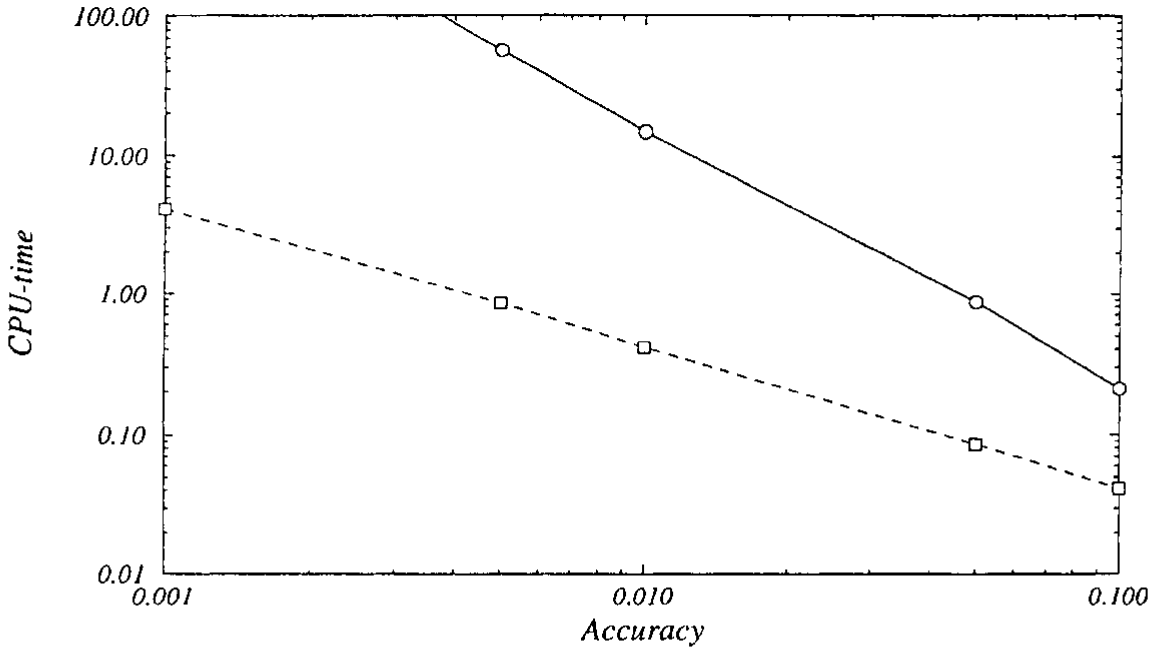
\includegraphics[width=.633\paperwidth]{images/fig-7-3-1.png}
  \caption{RT(1)(实线)和 BDM(2)(虚线)混合有限元的 CPU 用时与精度的关系}\label{fig:7.3.1}
\end{figure}

\clearpage
\section{更一般的约束问题的逼近}\label{sec:7.4}
\SourcePage{257}

本节介绍由\BookCite{babuska1971}{Babuška(1971)}和\BookCite{brezzi1974}{Brezzi(1974)}建立的抽象理论,讨论形如\eqref{eq:7.1.15}、\eqref{eq:7.1.16}的问题及其内逼近\eqref{eq:7.2.1}的解的存在性和唯一性.前面已经指出,若系数矩阵 \(\{a^{ij}\}\) 对称,这些问题等价于确定一个约束问题所对应的 Lagrange 泛函的唯一鞍点.以下分析无需这一对称性假设,所得结果也适用于更一般的问题.因此,这里在较广的意义上使用“约束问题”一词.

我们将沿用\BookCite{brezzi1974}{Brezzi(1974)}建立的理论.该理论推广并涵盖第~\ref{sec:7.2}~节只针对二阶椭圆方程\eqref{eq:7.1.1}给出的理论.事实上,对以速度 \(\boldsymbol{u}\) 和压力 \(p\) 为原始变量的 Stokes 问题作 Galerkin 逼近(见第~\BookRef{ch:9}{9}~章)时,便要用到下面的抽象理论.

更一般地说,多种边值问题的混合逼近都可以纳入这一抽象理论进行数值分析.例如,双调和算子 \(\Delta^2\) 的边值问题及其在板弯曲问题中的应用,以及采用流函数表述的 Stokes 和 Navier--Stokes 问题,都属于这种情形(见第~\BookRef{sec:10.4}{10.4}~节,亦见\BookCite{brezzi-fortin1991}{Brezzi 和 Fortin(1991)}第 IV 章).线性弹性问题的混合逼近是另一个例子(见\BookCite{brezzi-fortin1991}{Brezzi 和 Fortin(1991)}第 VII 章及其中所引文献).

\subsection{抽象表述}\label{sec:7.4.1}

先给出这一分析的一般框架.令 \(X\) 和 \(M\) 为两个实 Hilbert 空间,范数分别为 \(\|\cdot\|_X\) 和 \(\|\cdot\|_M\).设 \(X'\) 和 \(M'\) 为它们的对偶空间,即分别由 \(X\) 和 \(M\) 上的连续线性泛函组成的空间.引入两个双线性形式
\begin{equation}\label{eq:7.4.1}
  a(\cdot,\cdot)\colon X\times X\to\mathbb R,\qquad
  b(\cdot,\cdot)\colon X\times M\to\mathbb R,
\end{equation}
使对每个 \(w,v\in X\) 和 \(\mu\in M\),都有
\begin{equation}\label{eq:7.4.2}
  |a(w,v)|\le\gamma\|w\|_X\|v\|_X,\qquad
  |b(w,\mu)|\le\delta\|w\|_X\|\mu\|_M.
\end{equation}
考察下列约束问题：
\SourcePage{258}
\begin{equation}\label{eq:7.4.3}
  \left\{
  \begin{aligned}
    &\text{求 }(u,\eta)\in X\times M,\ \text{使}\\
    &a(u,v)+b(v,\eta)=\langle l,v\rangle&&\forall\,v\in X,\\
    &b(u,\mu)=\langle\sigma,\mu\rangle&&\forall\,\mu\in M,
  \end{aligned}
  \right.
\end{equation}
其中 \(l\in X'\)、\(\sigma\in M'\),\(\langle\cdot,\cdot\rangle\) 表示 \(X'\) 与 \(X\) 或 \(M'\) 与 \(M\) 之间的对偶配对.

将问题\eqref{eq:7.4.3}改写成算子形式会很方便.为双线性形式 \(a(\cdot,\cdot)\) 和 \(b(\cdot,\cdot)\) 分别引入算子 \(A\in\mathcal L(X;X')\) 和 \(B\in\mathcal L(X;M')\),其定义为
\begin{align}
  \langle Aw,v\rangle&=a(w,v)&&\forall\,w,v\in X,\label{eq:7.4.4}\\
  \langle Bv,\mu\rangle&=b(v,\mu)&&\forall\,v\in X,\ \mu\in M.\label{eq:7.4.5}
\end{align}
以 \(B^T\in\mathcal L(M;X')\) 表示 \(B\) 的伴随算子,即
\begin{equation}\label{eq:7.4.6}
  \langle B^T\mu,v\rangle=\langle Bv,\mu\rangle=b(v,\mu)
      \qquad\forall\,v\in X,\ \mu\in M.
\end{equation}
于是,可将\eqref{eq:7.4.3}写成求 \((u,\eta)\in X\times M\),使
\begin{equation}\label{eq:7.4.7}
  \begin{cases}
    Au+B^T\eta=l,&\text{在 }X'\text{ 中},\\
    Bu=\sigma,&\text{在 }M'\text{ 中}.
  \end{cases}
\end{equation}

现在定义仿射流形
\[
  X^\sigma:=\{v\in X\mid b(v,\mu)=\langle\sigma,\mu\rangle
      \quad\forall\,\mu\in M\}.
\]
显然,\(X^0=\ker B\) 是 \(X\) 的闭子空间.可以将问题\eqref{eq:7.4.3}与下列问题联系起来：
\begin{equation}\label{eq:7.4.8}
  \text{求 }u\in X^\sigma,\quad\text{使}\quad
    a(u,v)=\langle l,v\rangle\qquad\forall\,v\in X^0.
\end{equation}
容易看出,若 \((u,\eta)\) 是\eqref{eq:7.4.3}的解,则 \(u\) 是\eqref{eq:7.4.8}的解.下面将引入适当条件,使反过来也成立,并保证\eqref{eq:7.4.8}有唯一解,从而构造\eqref{eq:7.4.3}的解.

在此之前,需要证明一个关于双线性形式 \(b(\cdot,\cdot)\) 和算子 \(B\) 的等价性结论.记 \(X_\#^0\) 为 \(X^0\) 的极集,即
\begin{equation}\label{eq:7.4.9}
  X_\#^0:=\{g\in X'\mid\langle g,v\rangle=0\quad\forall\,v\in X^0\}.
\end{equation}
由于 \(X^0=\ker B\),也可写成 \(X_\#^0=(\ker B)_\#\).将 \(X\) 作如下分解：
\[
  X=X^0\oplus(X^0)^\perp.
\]
一般来说,\(\ker B=X^0\ne\{0\}\),因此 \(B\) 并非从 \(X\) 到 \(M'\) 的同构.下面要引入的一个条件等价于\SourcePage{259}\(B\) 从 \((X^0)^\perp\) 到 \(M'\) 是同构,并且 \(B^T\) 从 \(M\) 到 \(X_\#^0\) 是同构.

\begin{proposition}[]{7.4.1}
下列陈述等价：
\begin{enumerate}[label=\alph*.]
  \item 存在常数 \(\beta^*>0\),使相容性条件
  \begin{equation}\label{eq:7.4.10}
    \forall\,\mu\in M,\ \exists\,v\in X,\ v\ne0:\quad
      b(v,\mu)\ge\beta^*\|v\|_X\|\mu\|_M
  \end{equation}
  成立.
  \item 算子 \(B^T\) 是从 \(M\) 到 \(X_\#^0\) 的同构,并且
  \begin{equation}\label{eq:7.4.11}
    \|B^T\mu\|_{X'}:=\sup_{\substack{v\in X\\v\ne0}}
       \frac{\langle B^T\mu,v\rangle}{\|v\|_X}
         \ge\beta^*\|\mu\|_M\qquad\forall\,\mu\in M.
  \end{equation}
  \item 算子 \(B\) 是从 \((X^0)^\perp\) 到 \(M'\) 的同构,并且
  \begin{equation}\label{eq:7.4.12}
    \|Bv\|_{M'}:=\sup_{\substack{\mu\in M\\\mu\ne0}}
       \frac{\langle Bv,\mu\rangle}{\|\mu\|_M}
       \ge\beta^*\|v\|_X\qquad\forall\,v\in(X^0)^\perp.
  \end{equation}
\end{enumerate}
\end{proposition}

\begin{proof}
先证明 a. 与 b. 等价.由 \(B^T\) 的定义(见\eqref{eq:7.4.6})可知,\eqref{eq:7.4.10}和\eqref{eq:7.4.11}等价.因此,只需证明 \(B^T\) 是从 \(M\) 到 \(X_\#^0\) 的同构.显然,\eqref{eq:7.4.11}表明 \(B^T\) 从 \(M\) 到其值域 \(\mathcal R(B^T)\) 为单射,且逆算子连续.由此,\(\mathcal R(B^T)\) 是 \(X'\) 的闭子空间.只需证明 \(\mathcal R(B^T)=X_\#^0\).应用闭值域定理(例如,见\BookCite{yosida1974}{Yosida(1974)}第 205 页)立即得到
\[
  \mathcal R(B^T)=(\ker B)_\#=X_\#^0.
\]

接下来证明 b. 与 c. 等价.首先说明,\(X_\#^0\) 可与 \((X^0)^\perp\) 的对偶空间等同.事实上,对每个 \(g\in((X^0)^\perp)'\),可对应一个 \(\widehat g\in X'\),满足
\[
  \langle\widehat g,v\rangle=\langle g,P^\perp v\rangle\qquad\forall\,v\in X,
\]
其中 \(P^\perp\) 是到 \((X^0)^\perp\) 的正交投影.显然 \(\widehat g\in X_\#^0\),而且可以验证,\(g\mapsto\widehat g\) 是从 \(((X^0)^\perp)'\) 到 \(X_\#^0\) 的等距双射.因此,\(B^T\) 从 \(M\) 到 \(((X^0)^\perp)'\) 是同构且满足
\[
  \|(B^T)^{-1}\|_{\mathcal L(X_\#^0;M)}\le\frac1{\beta^*}
\]
的充要条件是,\(B\) 从 \((X^0)^\perp\) 到 \(M'\) 是同构且满足
\[
  \|B^{-1}\|_{\mathcal L(M';(X^0)^\perp)}\le\frac1{\beta^*}.
\]
证明完毕.\hfill\(\square\)
\end{proof}

\SourcePage{260}现在可以证明本节的主要定理.

\begin{theorem}[]{7.4.1}
假设双线性形式 \(a(\cdot,\cdot)\) 满足\eqref{eq:7.4.2},并在 \(X^0\) 上具有强制性,即存在常数 \(\alpha>0\),使
\begin{equation}\label{eq:7.4.13}
  a(v,v)\ge\alpha\|v\|_X^2\qquad\forall\,v\in X^0.
\end{equation}
还假设双线性形式 \(b(\cdot,\cdot)\) 满足\eqref{eq:7.4.2},且相容性条件\eqref{eq:7.4.10}成立.则对每个 \(l\in X'\)、\(\sigma\in M'\),\eqref{eq:7.4.8}有唯一解 \(u\),并且存在唯一的 \(\eta\in M\),使 \((u,\eta)\) 是\eqref{eq:7.4.3}的唯一解.此外,映射 \((l,\sigma)\mapsto(u,\eta)\) 是从 \(X'\times M'\) 到 \(X\times M\) 的同构,并且
\begin{align}
  \|u\|_X&\le\frac1\alpha
    \left(\|l\|_{X'}+\frac{\alpha+\gamma}{\beta^*}\|\sigma\|_{M'}\right),\label{eq:7.4.14}\\
  \|\eta\|_M&\le\frac1{\beta^*}
    \left[\left(1+\frac{\gamma}{\alpha}\right)\|l\|_{X'}
       +\frac{\gamma(\alpha+\gamma)}{\alpha\beta^*}\|\sigma\|_{M'}\right].\label{eq:7.4.15}
\end{align}
\end{theorem}

\begin{proof}
问题\eqref{eq:7.4.8}解的唯一性直接由强制性假设\eqref{eq:7.4.13}得到.

现在证明存在性.由于满足条件\eqref{eq:7.4.10},由命题~\ref{pro:7.4.1}的 c.,存在唯一的 \(u^0\in(X^0)^\perp\),使 \(Bu^0=\sigma\),且
\begin{equation}\label{eq:7.4.16}
  \|u^0\|_X\le\frac1{\beta^*}\|\sigma\|_{M'}.
\end{equation}
因此,可将\eqref{eq:7.4.8}改写为
\begin{equation}\label{eq:7.4.17}
  \text{求 }\widetilde u\in X^0,\quad\text{使}\quad
    a(\widetilde u,v)=\langle l,v\rangle-a(u^0,v)\qquad\forall\,v\in X^0,
\end{equation}
并令 \(u=\widetilde u+u^0\) 为\eqref{eq:7.4.8}的解.由 Lax--Milgram 引理(见定理~\ref{thm:5.1.1}),\eqref{eq:7.4.17}有唯一解,并且
\begin{equation}\label{eq:7.4.18}
  \|\widetilde u\|_X\le\frac1\alpha(\|l\|_{X'}+\gamma\|u^0\|_X).
\end{equation}

现在考察问题\eqref{eq:7.4.3}.由于\eqref{eq:7.4.17}可写成
\[
  \langle Au-l,v\rangle=0\qquad\forall\,v\in X^0,
\]
可知 \(Au-l\in X_\#^0\).再由命题~\ref{pro:7.4.1}的 b.,可以找到唯一的 \(\eta\in M\),使 \(Au-l=-B^T\eta\),即 \((u,\eta)\) 是\eqref{eq:7.4.3}的解,并满足
\begin{equation}\label{eq:7.4.19}
  \|\eta\|_M\le\frac1{\beta^*}\|Au-l\|_{X'}.
\end{equation}
\SourcePage{261}前面已指出,\eqref{eq:7.4.3}的每个解 \((u,\eta)\) 都给出\eqref{eq:7.4.8}的解 \(u\),所以问题\eqref{eq:7.4.3}的解也唯一.最后,合用不等式\eqref{eq:7.4.16}、\eqref{eq:7.4.18}和\eqref{eq:7.4.19},即得所需结论.\hfill\(\square\)
\end{proof}

现在可以考察抽象约束问题\eqref{eq:7.4.3}的逼近.设 \(X_h\) 和 \(M_h\) 分别为 \(X\) 和 \(M\) 的有限维子空间.给定 \(l\in X'\)、\(\sigma\in M'\),考虑求解下列问题：
\begin{equation}\label{eq:7.4.20}
  \left\{
  \begin{aligned}
    &\text{求 }(u_h,\eta_h)\in X_h\times M_h,\ \text{使}\\
    &a(u_h,v_h)+b(v_h,\eta_h)=\langle l,v_h\rangle&&\forall\,v_h\in X_h,\\
    &b(u_h,\mu_h)=\langle\sigma,\mu_h\rangle&&\forall\,\mu_h\in M_h.
  \end{aligned}
  \right.
\end{equation}
仿照无限维情形,定义空间
\[
  X_h^\sigma:=\{v_h\in X_h\mid b(v_h,\mu_h)=\langle\sigma,\mu_h\rangle
     \quad\forall\,\mu_h\in M_h\}.
\]
由于 \(M_h\) 一般是 \(M\) 的真子空间,\(X_h^\sigma\) 未必包含于 \(X^\sigma\).

与\eqref{eq:7.4.8}对应的有限维问题为
\begin{equation}\label{eq:7.4.21}
  \text{求 }u_h\in X_h^\sigma,\quad\text{使}\quad
    a(u_h,v_h)=\langle l,v_h\rangle\qquad\forall\,v_h\in X_h^0.
\end{equation}
显然,\eqref{eq:7.4.20}的每个解 \((u_h,\eta_h)\) 都给出\eqref{eq:7.4.21}的解 \(u_h\).下面将给出适当的条件,保证反过来也成立,并据此进行稳定性与收敛性分析.

\subsection{稳定性与收敛性分析}\label{sec:7.4.2}

先给出定理~\ref{thm:7.4.1}在有限维情形下的对应结果.它同时表明近似解 \((u_h,\eta_h)\) 的稳定性.

\begin{theorem}[稳定性]{7.4.2}
假定双线性形式 \(a(\cdot,\cdot)\) 满足\eqref{eq:7.4.2},并在 \(X_h^0\) 上具有强制性,即存在常数 \(\alpha_h>0\),使
\begin{equation}\label{eq:7.4.22}
  a(v_h,v_h)\ge\alpha_h\|v_h\|_X^2\qquad\forall\,v_h\in X_h^0.
\end{equation}
还假定双线性形式 \(b(\cdot,\cdot)\) 满足\eqref{eq:7.4.2}以及下列相容性条件：存在 \(\beta_h>0\),使
\begin{equation}\label{eq:7.4.23}
  \forall\,\mu_h\in M_h,\ \exists\,v_h\in X_h,\ v_h\ne0:\quad
     b(v_h,\mu_h)\ge\beta_h\|v_h\|_X\|\mu_h\|_M.
\end{equation}
则对每个 \(l\in X'\)、\(\sigma\in M'\),\eqref{eq:7.4.20}存在唯一解 \((u_h,\eta_h)\),且满足\eqref{eq:7.4.14}和\eqref{eq:7.4.15}中分别以 \(\alpha_h\) 和 \(\beta_h\) 代替 \(\alpha\) 和 \(\beta^*\) 所得的估计.若\eqref{eq:7.4.22}中的 \(\alpha_h\) 和\eqref{eq:7.4.23}中的 \(\beta_h\) 均与 \(h\) 无关,这便给出了 \((u_h,\eta_h)\) 的稳定性.
\end{theorem}

\SourcePage{262}
\begin{proof}
在定理~\ref{thm:7.4.1}中以 \(X_h\)、\(M_h\) 代替 \(X\)、\(M\),并注意到
\[
  \|l\|_{X_h'}\le\|l\|_{X'},\qquad \|\sigma\|_{M_h'}\le\|\sigma\|_{M'},
\]
即可得到上述结论.
\end{proof}
不过,必须注意,\(X_h^0\) 未必包含于 \(X^0\),因而\eqref{eq:7.4.13}并不蕴含\eqref{eq:7.4.22}.同样,由于 \(X_h\) 一般是 \(X\) 的真子空间,\eqref{eq:7.4.10}也不蕴含\eqref{eq:7.4.23}.

如第~\ref{sec:7.2.1}~节已指出的,相容性条件\eqref{eq:7.4.23}也称为 \emph{inf--sup 条件}或 \emph{Ladyzhenskaya--Babuška--Brezzi 条件}.

现在来看收敛性定理.它的证明与定理~\ref{thm:7.2.2}的证明很相似,这里仍将给出.

\begin{theorem}[收敛性]{7.4.3}
设定理~\ref{thm:7.4.1}和定理~\ref{thm:7.4.2}的假设均满足.则\eqref{eq:7.4.3}的解 \((u,\eta)\) 和\eqref{eq:7.4.20}的解 \((u_h,\eta_h)\) 满足下列误差估计：
\begin{align}
  \|u-u_h\|_X&\le\left(1+\frac{\gamma}{\alpha_h}\right)
      \inf_{v_h^*\in X_h^\sigma}\|u-v_h^*\|_X
      +\frac{\delta}{\alpha_h}\inf_{\mu_h\in M_h}\|\eta-\mu_h\|_M,\label{eq:7.4.24}\\
  \begin{split}
  \|\eta-\eta_h\|_M&\le\frac{\gamma}{\beta_h}\left(1+\frac{\gamma}{\alpha_h}\right)
      \inf_{v_h^*\in X_h^\sigma}\|u-v_h^*\|_X\\
      &\quad+\left(1+\frac{\delta}{\beta_h}+\frac{\gamma\delta}{\alpha_h\beta_h}\right)
      \inf_{\mu_h\in M_h}\|\eta-\mu_h\|_M.
  \end{split}\label{eq:7.4.25}
\end{align}
此外,还有估计
\begin{equation}\label{eq:7.4.26}
  \inf_{v_h^*\in X_h^\sigma}\|u-v_h^*\|_X
    \le\left(1+\frac{\delta}{\beta_h}\right)\inf_{v_h\in X_h}\|u-v_h\|_X.
\end{equation}
由\eqref{eq:7.4.24}至\eqref{eq:7.4.26}可知,只要\eqref{eq:7.4.22}和\eqref{eq:7.4.23}可用与 \(h\) 无关的常数成立,收敛就是最优的.
\end{theorem}

\begin{proof}
取 \(v_h\in X_h\)、\(v_h^*\in X_h^\sigma\) 和 \(\mu_h\in M_h\).将\eqref{eq:7.4.3}和\eqref{eq:7.4.20}的第一个方程相减,可得
\[
  a(u_h-v_h^*,v_h)+b(v_h,\eta_h-\mu_h)
     =a(u-v_h^*,v_h)+b(v_h,\eta-\mu_h).
\]
取 \(v_h=u_h-v_h^*\in X_h^0\),由\eqref{eq:7.4.22}和\eqref{eq:7.4.2}可得
\[
  \|u_h-v_h^*\|_X
     \le\frac1{\alpha_h}\bigl(\gamma\|u-v_h^*\|_X+\delta\|\eta-\mu_h\|_M\bigr),
\]
所以\eqref{eq:7.4.24}成立.

为得到\eqref{eq:7.4.25},从相容性条件\eqref{eq:7.4.23}出发.对每个 \(\mu_h\in M_h\),有
\SourcePage{263}
\[
  \|\eta_h-\mu_h\|_M
    \le\frac1{\beta_h}\sup_{\substack{v_h\in X_h\\v_h\ne0}}
       \frac{b(v_h,\eta_h-\mu_h)}{\|v_h\|_X}.
\]
另一方面,由\eqref{eq:7.4.3}和\eqref{eq:7.4.20}的第一个方程相减可知
\[
  b(v_h,\eta_h-\mu_h)=a(u-u_h,v_h)+b(v_h,\eta-\mu_h).
\]
由\eqref{eq:7.4.2}得到
\[
  \|\eta_h-\mu_h\|_M
    \le\frac1{\beta_h}\bigl(\gamma\|u-u_h\|_X+\delta\|\eta-\mu_h\|_M\bigr).
\]
结合\eqref{eq:7.4.24},即可得到\eqref{eq:7.4.25}.

最后,证明\eqref{eq:7.4.26}.对于每个 \(v_h\in X_h\),由\eqref{eq:7.4.23}和命题~\ref{pro:7.4.1}可知,存在唯一的 \(z_h\in X_h\cap(X_h^0)^\perp\),使
\[
  b(z_h,\mu_h)=b(u-v_h,\mu_h)\qquad\forall\,\mu_h\in M_h,
\]
并且
\[
  \|z_h\|_X\le\frac{\delta}{\beta_h}\|u-v_h\|_X.
\]
令 \(v_h^*:=z_h+v_h\).由于对每个 \(\mu_h\in M_h\) 都有 \(b(u,\mu_h)=\langle\sigma,\mu_h\rangle\),显然 \(v_h^*\in X_h^\sigma\).此外,
\[
  \|u-v_h^*\|_X\le\|u-v_h\|_X+\|z_h\|_X
    \le\left(1+\frac{\delta}{\beta_h}\right)\|u-v_h\|_X.
\]
于是\eqref{eq:7.4.26}成立.\hfill\(\square\)
\end{proof}

\begin{note}\NumberedNote{note:7.4.1}
考察定理~\ref{thm:7.2.2}的证明,特别是\eqref{eq:7.2.17},可看出,在 \(X_h^0\subset X^0\) 的条件下,只用 \(\inf_{v_h\in X_h}\|u-v_h\|_X\) 即可估计 \(\|u-u_h\|_X\).此外,即使相容性条件\eqref{eq:7.4.10}和\eqref{eq:7.4.23}不成立,误差估计\eqref{eq:7.4.24}仍然成立.\hfill\(\square\)
\end{note}

\begin{note}\NumberedNote{note:7.4.2}{\heiti(伪模态)}
相容性条件\eqref{eq:7.4.23}是保证 \(\eta_h\) 唯一的必要条件.事实上,它可以写成：若 \(\mu_h\in M_h\),并且对每个 \(v_h\in X_h\) 都有 \(b(v_h,\mu_h)=0\),则 \(\mu_h=0\).

所以,若\eqref{eq:7.4.23}不成立,则存在非零的 \(\mu_h^*\in M_h\),使
\[
  b(v_h,\mu_h^*)=0\qquad\forall\,v_h\in X_h.
\]
因此,若 \((u_h,\eta_h)\) 是\eqref{eq:7.4.20}的解,则对每个 \(\tau\in\mathbb R\),\((u_h,\eta_h+\tau\mu_h^*)\) 也是同一个问题的解.

任何这样的 \(\mu_h^*\) 都称为{\heiti 伪模态}(或{\heiti 寄生模态}),因为数值问题\eqref{eq:7.4.20}无法检测到它.因而它可能使方法不稳定(另见第~\BookRef{sec:9.2.2}{9.2.2}~节).\hfill\(\square\)
\end{note}

\subsection{如何验证一致相容性条件}\label{sec:7.4.3}
\SourcePage{264}

在大多数应用中,验证\eqref{eq:7.4.22}关于 \(h\) 一致成立并不困难,例如见第~\ref{sec:7.2.1}~节和第~\BookRef{ch:9}{9}~章.较困难的是证明相容性条件\eqref{eq:7.4.23}关于 \(h\) 一致成立.

\BookCite{fortin1977}{Fortin(1977)}提出了这方面的第一个判据(见引理~\ref{lem:7.2.1}).这里给出一般的抽象表述,其证明思路与前面相同.

\begin{lemma}[Fortin]{7.4.1}
假设相容性条件\eqref{eq:7.4.10}成立,并且存在算子 \(\tau_h\colon X\to X_h\),使
\[
  \begin{aligned}
    \text{(i)}\quad &b(v-\tau_h(v),\mu_h)=0 &&\forall\,v\in X,\ \mu_h\in M_h,\\
    \text{(ii)}\quad &\|\tau_h(v)\|_X\le C_*\|v\|_X &&\forall\,v\in X,
  \end{aligned}
\]
其中 \(C_*>0\) 与 \(h\) 无关.则相容性条件\eqref{eq:7.4.23}成立,且可取 \(\beta=\beta^*/C_*\).
\end{lemma}

另一种值得考察的情形是取 \(X=(H_0^1(\Omega))^d\)、\(M=L_0^2(\Omega)\),并令 \(a(\boldsymbol{w},\boldsymbol{v})=\nu(\nabla\boldsymbol{w},\nabla\boldsymbol{v})\)、\(b(\boldsymbol{v},q)=-(q,\operatorname{div}\boldsymbol{v})\),其中 \(\nu>0\).这些是 Stokes 问题变分形式中的函数空间和双线性形式(见第~\BookRef{ch:9}{9}~章).在这种情形下,\BookCite{verfurth1984b}{Verfürth(1984b)}证明了下列结果.

\begin{lemma}[Verfürth]{7.4.2}
设 \(\mathcal T_h\) 是 \(\overline\Omega\) 的一族拟一致剖分.假设 \(M_h\subset H^1(\Omega)\cap L_0^2(\Omega)\),且存在 \(\widehat\beta>0\),使
\begin{equation}\label{eq:7.4.27}
  \forall\,q_h\in M_h,\ \exists\,\boldsymbol{v}_h\in X_h,\ \boldsymbol{v}_h\ne0:\quad
     b(\boldsymbol{v}_h,q_h)\ge\widehat\beta\|\boldsymbol{v}_h\|_0\|q_h\|_1.
\end{equation}
再假设存在算子 \(R_h\colon X\to X_h\) 和常数 \(K>0\),使
\begin{equation}\label{eq:7.4.28}
  \|\boldsymbol{v}-R_h(\boldsymbol{v})\|_0+h\|\boldsymbol{v}-R_h(\boldsymbol{v})\|_1
     \le Kh|\boldsymbol{v}|_1\qquad\forall\,\boldsymbol{v}\in X.
\end{equation}
则相容性条件\eqref{eq:7.4.23}关于 \(h\) 一致成立.
\end{lemma}

\begin{proof}
首先,由逆不等式\eqref{eq:6.3.21}可知,对每个 \(\boldsymbol{v}_h\in X_h\),都有
\[
  \|\boldsymbol{v}_h\|_1\le Ch^{-1}\|\boldsymbol{v}_h\|_0.
\]
因此,条件\eqref{eq:7.4.27}蕴含
\begin{equation}\label{eq:7.4.29}
  \forall\,q_h\in M_h,\ \exists\,\boldsymbol{v}_h\in X_h,\ \boldsymbol{v}_h\ne0:\quad
     b(\boldsymbol{v}_h,q_h)\ge K_1h\|\boldsymbol{v}_h\|_1\|q_h\|_1.
\end{equation}
回顾一下,对每个 \(q_h\in M_h\),都存在 \(\boldsymbol{w}\in X\),使 \(\operatorname{div}\boldsymbol{w}=-q_h\),并且
\begin{equation}\label{eq:7.4.30}
  \|\boldsymbol{w}\|_1\le K_2\|q_h\|_0
\end{equation}
\SourcePage{265}(例如,见\BookCite{girault-raviart1986}{Girault 和 Raviart(1986)}第 24 页).于是,由\eqref{eq:7.4.28}得到
\begin{equation}\label{eq:7.4.31}
  \begin{aligned}
    \|R_h(\boldsymbol{w})\|_1
      &\le\|R_h(\boldsymbol{w})-\boldsymbol{w}\|_1+\|\boldsymbol{w}\|_1\\
      &\le(1+K)\|\boldsymbol{w}\|_1\le K_2(1+K)\|q_h\|_0.
  \end{aligned}
\end{equation}
若 \(q_h\) 满足
\begin{equation}\label{eq:7.4.32}
  \|q_h\|_0\le KK_2h\|q_h\|_1,
\end{equation}
则由\eqref{eq:7.4.29}可得
\begin{equation}\label{eq:7.4.33}
  b(\boldsymbol{v}_h,q_h)\ge\frac{K_1}{KK_2}\|\boldsymbol{v}_h\|_1\|q_h\|_0.
\end{equation}
若
\begin{equation}\label{eq:7.4.34}
  \|q_h\|_0>KK_2h\|q_h\|_1,
\end{equation}
则由\eqref{eq:7.4.28}、\eqref{eq:7.4.30}和\eqref{eq:7.4.31}得到
\begin{equation}\label{eq:7.4.35}
  \begin{aligned}
    b(R_h(\boldsymbol{w}),q_h)
      &=b(\boldsymbol{w},q_h)+b(R_h(\boldsymbol{w})-\boldsymbol{w},q_h)\\
      &\ge\|q_h\|_0^2-\|R_h(\boldsymbol{w})-\boldsymbol{w}\|_0\|q_h\|_1\\
      &\ge\|q_h\|_0^2-KK_2h\|q_h\|_0\|q_h\|_1\\
      &\ge\frac{1}{K_2(1+K)}
         (\|q_h\|_0-KK_2h\|q_h\|_1)\|R_h(\boldsymbol{w})\|_1.
  \end{aligned}
\end{equation}
其中 \(b(R_h(\boldsymbol{w})-\boldsymbol{w},q_h)\) 一项用了分部积分.

结合\eqref{eq:7.4.29}和\eqref{eq:7.4.35},容易证明,对每个满足\eqref{eq:7.4.34}的 \(q_h\in M_h\),都存在 \(\boldsymbol{z}_h\in X_h\)、\(\boldsymbol{z}_h\ne0\),使
\begin{equation}\label{eq:7.4.36}
  b(\boldsymbol{z}_h,q_h)\ge Q(h\|q_h\|_1)\|\boldsymbol{z}_h\|_1,
\end{equation}
其中
\[
  Q(\xi):=\max\left\{K_1\xi,\frac{1}{K_2(1+K)}
       (\|q_h\|_0-KK_2\xi)\right\},\qquad \xi>0.
\]
最后,求 \(Q(\xi)\) 在 \(\xi>0\) 上的最小值.由\eqref{eq:7.4.33}和\eqref{eq:7.4.36},可知\eqref{eq:7.4.23}成立,且可取
\[
  \beta=K_1K_2^{-1}[K_1(1+K)+K]^{-1}.
\]
\hfill\(\square\)
\end{proof}

注意,\eqref{eq:7.4.27}与\eqref{eq:7.4.23}不同,其右端使用的是另一组范数.已有证明表明,一些常用于逼近 Stokes 问题的有限元空间满足\eqref{eq:7.4.27}.例如,第~\BookRef{sec:9.3.2}{9.3.2}~节将介绍 Taylor--Hood 单元和 Bercovier--Pironneau 单元,其证明分别见\BookCite{fortin1993}{Fortin(1993)}和\BookCite{bercovier-pironneau1979}{Bercovier 和 Pironneau(1979)}.

此外,在适当假设下,多种 \(X_h\) 都满足逼近性质\eqref{eq:7.4.28},例如见\eqref{eq:3.5.22}或\BookCite{clement1975}{Clément(1975)}.

\SourcePage{266}对于 Stokes 问题,还有一些可用来验证一致相容性条件\eqref{eq:7.4.23}的判据,由\BookCite{boland-nicolaides1983}{Boland 和 Nicolaides(1983)}及\BookCite{stenberg1984}{Stenberg(1984)}提出(另见\BookCite{gunzburger1989}{Gunzburger(1989)}第 16–21 页和\BookCite{girault-raviart1986}{Girault 和 Raviart(1986)}第 129–132 页).这些判据的基本做法是将 \(\Omega\) 划分成若干宏单元,只在各个宏单元上局部验证相容性条件\eqref{eq:7.4.23}.

\section{补充说明}\label{sec:7.5}

对于混合方法,已有关于 \(u-u_h\) 在 \(L^\infty(\Omega)\) 范数下的误差估计,例如见\BookCite{scholz1977}{Scholz(1977)}、\BookCite{douglas-roberts1985}{Douglas 和 Roberts(1985)}及\BookCite{gastaldi-nochetto1987}{Gastaldi 和 Nochetto(1987)}.

把本章的结果推广到一般的椭圆型算子
\[
  Lw:=-\sum_{i,j=1}^d D_i(a_{ij}D_jw)+\sum_{i=1}^d c_iD_iw+a_0w
\]
时可能遇到一些困难.对偶混合表述的情形见\BookCite{douglas-roberts1985}{Douglas 和 Roberts(1985)}的分析.

另一种推广涉及可写成如下形式的问题：
\[
  \left\{
  \begin{aligned}
    &\text{求 }(u,\eta)\in X\times M,\ \text{使}\\
    &a(u,v)+b(v,\eta)=\langle l,v\rangle&&\forall\,v\in X,\\
    &b(u,\mu)-d(\eta,\mu)=\langle\sigma,\mu\rangle&&\forall\,\mu\in M,
  \end{aligned}
  \right.
\]
其中 \(d(\cdot,\cdot)\) 是 \(M\times M\) 上连续且非负的双线性形式.关于该问题的分析,见\BookCite{roberts-thomas1991}{Roberts 和 Thomas(1991)},另见第~\BookRef{sec:9.6.7}{9.6.7}~节.

Brezzi 理论的另一项推广涉及下列问题：
\[
  \left\{
  \begin{aligned}
    &\text{求 }(u,\eta)\in X\times M,\ \text{使}\\
    &a(u,v)+b_1(v,\eta)=\langle l,v\rangle&&\forall\,v\in X,\\
    &b_2(u,\mu)=\langle\sigma,\mu\rangle&&\forall\,\mu\in M,
  \end{aligned}
  \right.
\]
其中双线性形式 \(b_1\) 和 \(b_2\) 彼此不同.见\BookCite{nicolaides1982}{Nicolaides(1982)}及\BookCite{bernardi-canuto-maday1988}{Bernardi、Canuto 和 Maday(1988)},后一项工作以 Stokes 问题的 Chebyshev 逼近为出发点.
